% Multinational Firms and Trade in Latin America -- WP_paper (the working paper)
% Overleaf project exported 2026-09-24 from the build of 2026-09-23 (stylized_facts/python/wp_export_overleaf.py).
% Compile with pdfLaTeX, the Overleaf default. Figures are in figures/<scope>/ and tables in tables/<scope>/,
% where <scope> is the sample: all = all goods; agro, manufacturing, mining, rest = the sectors;
% sectors = exhibits that compare the sectors. Each figure and table below starts with a '% ----' line.
\documentclass[11pt,a4paper]{article}
\usepackage[utf8]{inputenc}
\usepackage[T1]{fontenc}
\usepackage{mathptmx}
\usepackage[margin=2.5cm]{geometry}
\usepackage{graphicx,booktabs,amsmath,amssymb,adjustbox,float,caption,hyperref,xcolor,enumitem}
\captionsetup{font=small,labelfont=bf,skip=4pt}
\hypersetup{colorlinks,linkcolor=blue!50!black,urlcolor=blue!50!black,citecolor=blue!50!black}
\setlength{\parskip}{3pt}
\newcommand{\tbw}[1]{\textcolor{gray}{\textit{#1}}}
\title{\textbf{Multinational Firms and Trade in Latin America}\\[6pt]\large Six Stylized Facts on Ownership and Exports}
\author{Ignacio Marra de Arti\~nano\thanks{Universit\'e Libre de Bruxelles (ECARES).}
 \and Gabriel Scattolo\thanks{Inter-American Development Bank.}
 \and Sebasti\'an Vel\'asquez\thanks{Inter-American Development Bank.}
 \and Christian Volpe Martincus\thanks{Inter-American Development Bank and CESifo. The views and
interpretations in this paper are strictly those of the authors and should not be attributed to
the Inter-American Development Bank, its executive directors, or its member countries.}}
\date{This version: September 2026 \\[2pt] \small Preliminary draft, please do not circulate}
\begin{document}
\maketitle
\thispagestyle{empty}
\begin{abstract}\noindent We match the customs export records of nine Latin American countries to the ownership records of
Orbis and Dun \& Bradstreet and classify every exporter as a foreign multinational affiliate, a
domestic multinational affiliate or a local firm. Multinational affiliates account for 61 percent
of the region's exports, most of it foreign owned. Foreign affiliates concentrate in complex and
differentiated products, domestic ones in primary goods. The parents come from a few countries,
and a small number of large groups accounts for most of the value. Product--destination pairs with
more multinationals export more, and distance reduces the exports of multinationals less than
those of other firms. US groups are the only large investors that ship a sizeable share of their
affiliates' exports to their own country: 22 percent, against less than 3 percent for British,
Dutch or Swiss groups.
\end{abstract}
\vspace{4pt}
\noindent\textbf{Keywords:} Multinational Firms, Foreign Direct Investment, Exports, Ownership, Firm-Level Data, Latin America \\
\noindent\textbf{JEL codes:} F14, F23, D22, L25
\clearpage
\tableofcontents
\clearpage

\section{Introduction}\label{sec:intro}
Customs records show what a country exports and where, but not who owns the exporter. In Latin
America many exporters are affiliates of groups headquartered abroad, so this is a large gap.
Foreign direct investment statistics do not fill it: they show where capital goes, not which
firms export which products to which markets.

In this paper we match the customs export records of nine countries (Argentina, Chile, Colombia,
Costa Rica, the Dominican Republic, El Salvador, Paraguay, Peru and Uruguay) to the ownership
records of Orbis and Dun \& Bradstreet. Every exporter is classified as a foreign multinational
affiliate, a domestic multinational affiliate or a local firm, and the exports of foreign
affiliates can be traced to the country of their parent.

The data show six facts. First, multinational affiliates account for 61 percent of the region's
exports, from 47 percent in Peru to 74 percent in Colombia, and most of it is foreign owned.
Second, foreign affiliates concentrate in complex and differentiated products and domestic
multinationals in primary goods, especially within manufacturing. Third, the parents come from a
few countries: the United States, the United Kingdom and Canada account for half of
foreign-affiliate exports. Fourth, parents with more than 100 affiliates worldwide are 9 percent of
all parents and account for 56 percent of foreign-affiliate exports. Fifth, product--destination
pairs with more multinationals export more, and the relationship is about three times stronger for
foreign than for domestic affiliates, also for the exports of local firms. Sixth, distance reduces
the exports of multinationals less than those of other firms.

The United States deserves separate attention because it is both the largest parent country and
the largest destination. Affiliates of US groups account for 10.8 percent of the exports of the
nine countries, the United States buys 18.4 percent of them, and the two overlap in 2.5 percent.
US groups are the only large investors that ship a sizeable share of their affiliates' exports to
their own country: 22.3 percent, against 0.6 percent for British groups, 2.2 percent for Dutch
groups and almost none for Swiss or Liechtenstein groups. These shipments are concentrated in
Central America and the Caribbean, where US-parent affiliates account for 41 percent of El
Salvador's exports to the United States, 40 percent of Costa Rica's and 26 percent of the
Dominican Republic's. Groups from other countries follow different patterns. British and
Liechtenstein groups, mostly in mining, sell to Asia, and German and Japanese groups export from
Argentina to Brazil.

\tbw{Contribution to the literature: to be written.}

Section~\ref{sec:lit} reviews the literature, Section~\ref{sec:data} describes the data and
Section~\ref{sec:facts} presents the six facts. Section~\ref{sec:products} looks at products,
Section~\ref{sec:model} outlines the model and Section~\ref{sec:concl} concludes.


\section{Related Literature}\label{sec:lit}
\tbw{To be written. Three strands: firm-level evidence on multinational production and trade;
ownership, market power and trade policy; and evidence on multinational firms in Latin America.}


\section{Data}\label{sec:data}
\subsection{Customs data}

The export records come from the customs authorities of the nine countries. Each record gives the
value exported (FOB, US dollars) by a firm, of an HS6 product (2007 revision), to a destination, in
a year. Firms are identified by their tax number and name. The records cover all merchandise
exports in the years available for each country: Argentina 2011--2019, Chile 2009--2022, Colombia
2010--2021, Costa Rica 2010--2019, the Dominican Republic 2012--2019, El Salvador 2006--2018,
Paraguay 2012--2020, Peru 2010--2019 and Uruguay 2010--2019.

\subsection{Ownership data and matching}

Ownership comes from Orbis (Bureau van Dijk) and Dun \& Bradstreet, which report for each company
its global ultimate owner and the owner's country. We combine the two sources into one file with
the group, the country of the parent and the number of affiliates the group has worldwide.

Exporters are matched to this file in four steps: by tax number where the corporate records
report it; by company name within each country, using a character-based similarity measure,
with each candidate pair reviewed by a large language model; by company name across all countries; and, for the 500
largest unmatched exporters of each country, by hand, using company websites and business
registries. The tax number delivers about 60 percent of matched export value. After matching, the
parent's country is known for 92.5 percent of the export value of foreign affiliates.

\subsection{Definitions}

An exporter found in Orbis or Dun \& Bradstreet is a multinational affiliate (MNE). It is a
\emph{domestic} MNE when its ultimate parent is located in the exporting country and a
\emph{foreign} MNE otherwise; matched exporters without a recorded parent country are counted as
foreign. Exporters not found in either database are \emph{local} firms. Because the match relies
on ownership links, a group's head company exporting from its own country cannot be identified
and appears among local firms.

Products are classified with the Product Complexity Index of Hausmann and Hidalgo, the technology
classes of Lall (2000), the Rauch (1999) classification, and the end-use classes of BEC Rev.\,4.
Sectors are defined on HS chapters: agriculture 01--24, mining and fuels 25--27 and 71,
manufacturing 28--97 excluding 71. Distance comes from the CEPII gravity database.

\subsection{Sample}

Table~\ref{tab:p_sample} describes the sample by country and Table~\ref{tab:p_counts} summarizes
it. The nine countries have 165,543 exporters, of which 31,350 are matched to a corporate record.
They export 5,930 HS6 products to 253 destinations. The matched exporters belong to 17,094 groups
with parents in 165 countries.

% ---- Table: Sample Coverage, by Exporting Country
\begin{table}[H]\centering\footnotesize%
  \caption{Sample Coverage, by Exporting Country}%
  \label{tab:p_sample}%
  \adjustbox{max width=\textwidth, max totalheight=0.8\textheight}{\begin{tabular}{llrrrrrr}
\toprule
Origin & Years & Exporters & Matched & HS6 lines & Destinations & Records & Value (US\$bn/yr) \\
\midrule
ARG & 2011--2019 & 22,980 & 6,687 & 4,657 & 202 & 1,105,127 & 66.4 \\
COL & 2010--2021 & 47,711 & 7,711 & 4,850 & 223 & 1,164,935 & 44.0 \\
PER & 2010--2019 & 27,286 & 4,696 & 4,600 & 215 & 845,003 & 41.4 \\
CHL & 2009--2022 & 17,430 & 5,776 & 4,673 & 205 & 589,227 & 34.2 \\
CRI & 2010--2019 & 14,816 & 1,387 & 4,452 & 197 & 530,375 & 10.5 \\
DOM & 2012--2019 & 15,832 & 1,671 & 3,970 & 206 & 329,133 & 8.6 \\
PRY & 2012--2020 & 3,220 & 999 & 2,801 & 168 & 60,188 & 7.3 \\
URY & 2010--2019 & 5,828 & 1,465 & 3,611 & 208 & 121,452 & 7.0 \\
SLV & 2006--2018 & 10,440 & 958 & 4,310 & 183 & 362,774 & 5.0 \\
\midrule
All nine & 2006--2022 & 165,543 & 31,350 & 5,930 & 253 & 5,108,214 & 224.5 \\
\bottomrule
\end{tabular}
}%
  \par\vspace{3pt}%
  \begin{minipage}{0.95\textwidth}\footnotesize %
  \textit{Notes:} Exporters are distinct tax identifiers within each country; matched exporters are those found in Orbis or Dun \& Bradstreet. Records are firm--destination--HS6--year observations. Values are annual averages in US\$ billion.\\[3pt]%
  \textit{Source:} Authors' calculations based on customs data matched to Orbis and Dun \& Bradstreet.%
  \end{minipage}%
  \end{table}
% ---- Table: Sample Summary
\begin{table}[H]\centering\small%
  \caption{Sample Summary}%
  \label{tab:p_counts}%
  \adjustbox{max width=\textwidth, max totalheight=0.8\textheight}{\begin{tabular}{lr}
\toprule
Statistic & Value \\
\midrule
Exporting countries & 9 \\
Years & 2006--2022 \\
Records (firm $\times$ destination $\times$ HS6 $\times$ year) & 5,108,214 \\
Exporters & 165,543 \\
\quad matched to Orbis / Dun \& Bradstreet & 31,350 \\
HS6 product lines & 5,930 \\
Destination markets & 253 \\
Parent countries of foreign multinationals & 165 \\
Multinational groups & 17,094 \\
\midrule
Export value, all years (US\$ billion) & 2,394 \\
\quad foreign multinationals & 46.3\% \\
\quad domestic multinationals & 14.1\% \\
\quad local firms & 39.5\% \\
Foreign-MNE value with a recorded parent country & 92.5\% \\
\bottomrule
\end{tabular}
}%
  \par\vspace{3pt}%
  \begin{minipage}{0.95\textwidth}\footnotesize %
  \textit{Notes:} Nine countries, all available years pooled. Shares are percent of total export value.\\[3pt]%
  \textit{Source:} Authors' calculations based on customs data matched to Orbis and Dun \& Bradstreet.%
  \end{minipage}%
  \end{table}

\section{Six Stylized Facts}\label{sec:facts}

\subsection{Fact 1: Multinationals Account for a Large Share of Exports}
Figure~\ref{fig:p_f1} shows the share of each country's exports accounted for by multinational
affiliates. It ranges from 47 percent in Peru to 74 percent in Colombia and is 61 percent for the
nine countries together. Foreign affiliates account for 46 percent of total exports and domestic
multinationals for 14 percent. Foreign affiliates export more than domestic multinationals in every
country except Colombia, where the state oil company and its subsidiaries are domestic
multinationals. Chile, with copper and pulp, is the other country with a large domestic share.

Figures~\ref{fig:p_us3_total} and~\ref{fig:p_us3_origin} and Table~\ref{tab:p_us3_tab} separate
the two roles of the United States. The United States buys 18.4 percent of the region's exports
and US-parent affiliates ship 10.8 percent, but only 2.5 percent is both. US-parent affiliates
account for 13.6 percent of the region's exports to the United States, and for much more in El
Salvador, Costa Rica and the Dominican Republic.

% ---- Figure: Multinational Share of Export Value, by Exporting Country
\begin{figure}[H]\centering%
  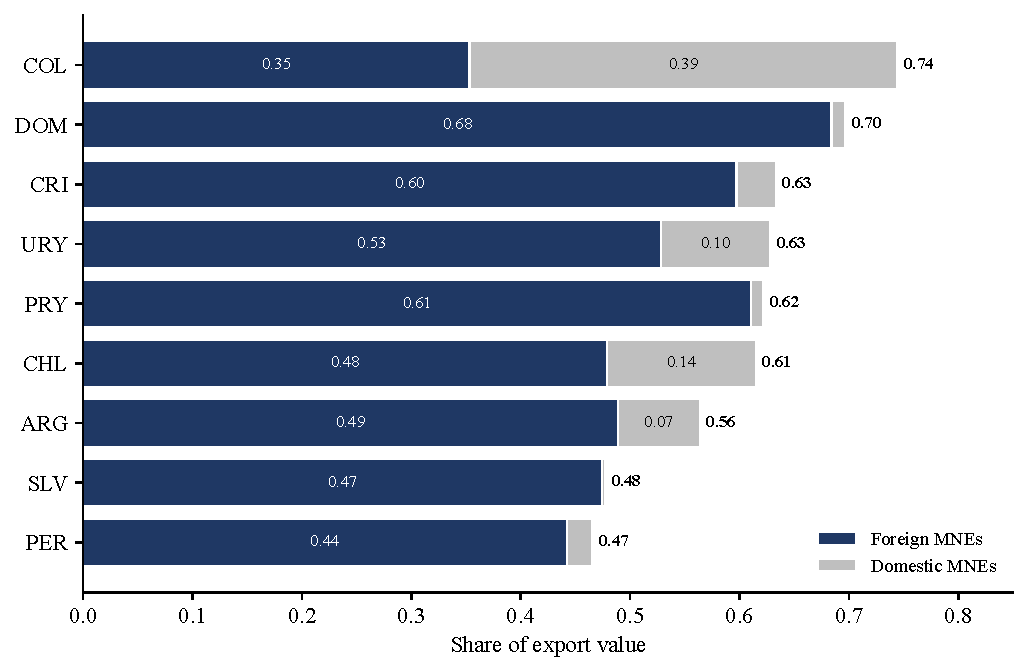
\includegraphics[width=0.8\textwidth,height=0.8\textheight,keepaspectratio]{figures/all/fig_wp0_fig1_origin.pdf}%
  \caption{Multinational Share of Export Value, by Exporting Country}%
  \label{fig:p_f1}%
  \par\vspace{2pt}%
  \parbox{0.92\textwidth}{\footnotesize %
  \textit{Notes:} Shares of export value, all available years pooled. The figure at the end of each bar is the total MNE share.\\[3pt]%
  \textit{Source:} Authors' calculations based on customs data matched to Orbis and Dun \& Bradstreet.}%
  \end{figure}
% ---- Figure: Exports to the United States and Exports by US-Parent Multinationals
\begin{figure}[H]\centering%
  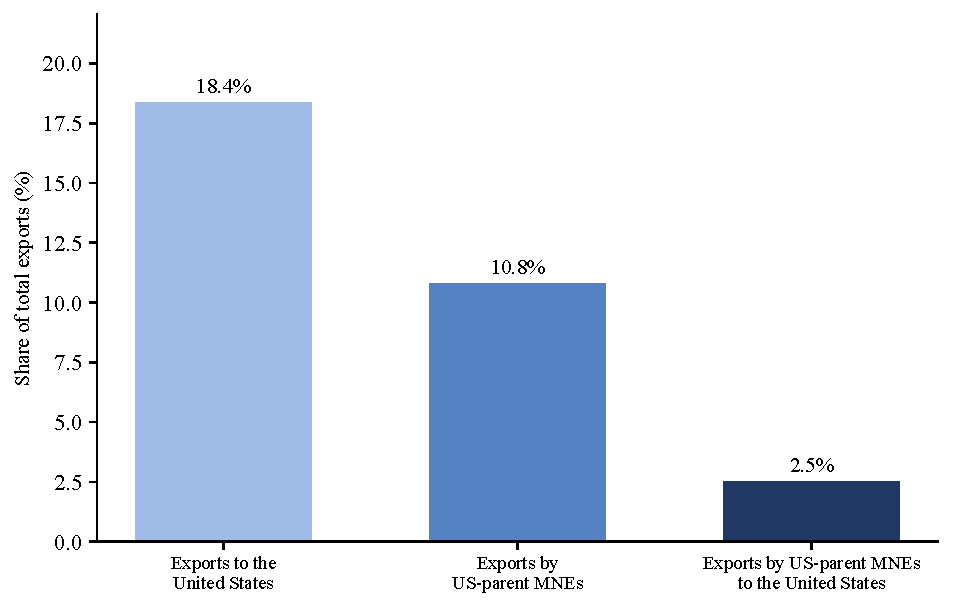
\includegraphics[width=0.6\textwidth,height=0.8\textheight,keepaspectratio]{figures/all/fig_wp3_us_three_shares_total.pdf}%
  \caption{Exports to the United States and Exports by US-Parent Multinationals}%
  \label{fig:p_us3_total}%
  \par\vspace{2pt}%
  \parbox{0.92\textwidth}{\footnotesize %
  \textit{Notes:} Shares of the total exports of the nine countries. The third bar is exports by US-parent MNEs shipped to the United States.\\[3pt]%
  \textit{Source:} Authors' calculations based on customs data matched to Orbis and Dun \& Bradstreet.}%
  \end{figure}
% ---- Figure: Exports to the United States and Exports by US-Parent Multinationals, by Exporting Country
\begin{figure}[H]\centering%
  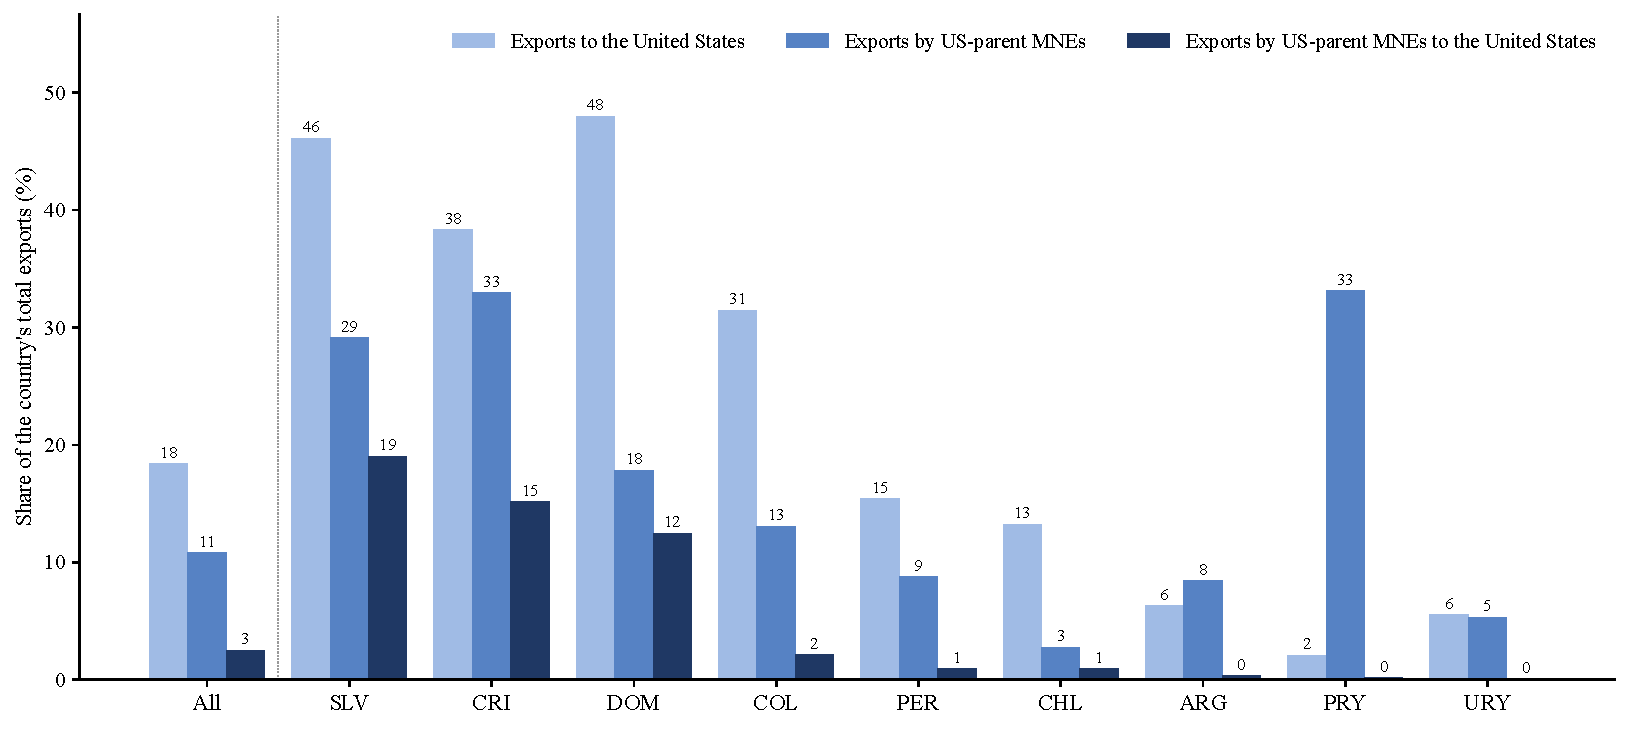
\includegraphics[width=1.0\textwidth,height=0.8\textheight,keepaspectratio]{figures/all/fig_wp3_us_three_shares_origin.pdf}%
  \caption{Exports to the United States and Exports by US-Parent Multinationals, by Exporting Country}%
  \label{fig:p_us3_origin}%
  \par\vspace{2pt}%
  \parbox{0.92\textwidth}{\footnotesize %
  \textit{Notes:} Shares of each country's total exports.\\[3pt]%
  \textit{Source:} Authors' calculations based on customs data matched to Orbis and Dun \& Bradstreet.}%
  \end{figure}
% ---- Table: Exports to the United States and Exports by US-Parent Multinationals, by Exporting Country
\begin{table}[H]\centering\small%
  \caption{Exports to the United States and Exports by US-Parent Multinationals, by Exporting Country}%
  \label{tab:p_us3_tab}%
  \adjustbox{max width=\textwidth, max totalheight=0.8\textheight}{\begin{tabular}{lrrrrr}
\toprule
Origin & \multicolumn{1}{p{2.3cm}}{\raggedright (1) \% of exports going to the USA} & \multicolumn{1}{p{2.3cm}}{\raggedright (2) \% of exports carried by US-parent MNEs} & \multicolumn{1}{p{2.6cm}}{\raggedright (3) \% of exports carried by US-parent MNEs and going to the USA} & \multicolumn{1}{p{2.6cm}}{\raggedright (4) = (3)/(1): US-parent share of the exports going to the USA (\%)} & \multicolumn{1}{p{1.8cm}}{\raggedright Total exports (US\$bn/yr)} \\
\midrule
All & 18.4 & 10.8 & 2.5 & 13.6 & 224.5 \\
\midrule
SLV & 46.1 & 29.1 & 19.0 & 41.3 & 5.0 \\
CRI & 38.3 & 33.0 & 15.1 & 39.5 & 10.5 \\
DOM & 48.0 & 17.8 & 12.5 & 26.0 & 8.6 \\
COL & 31.5 & 13.1 & 2.1 & 6.8 & 44.0 \\
PER & 15.4 & 8.8 & 0.9 & 6.0 & 41.4 \\
CHL & 13.3 & 2.8 & 0.9 & 6.9 & 34.2 \\
ARG & 6.3 & 8.4 & 0.3 & 5.5 & 66.4 \\
PRY & 2.1 & 33.1 & 0.2 & 8.1 & 7.3 \\
URY & 5.5 & 5.3 & 0.0 & 0.4 & 7.0 \\
\bottomrule
\end{tabular}
}%
  \par\vspace{3pt}%
  \begin{minipage}{0.95\textwidth}\footnotesize %
  \textit{Notes:} Columns (1)--(3): percent of each country's total exports. Column (4): percent of exports to the United States shipped by US-parent MNEs. Countries sorted by column (3). Values are annual averages in US\$ billion.\\[3pt]%
  \textit{Source:} Authors' calculations based on customs data matched to Orbis and Dun \& Bradstreet.%
  \end{minipage}%
  \end{table}

\subsection{Fact 2: Foreign Multinationals Specialize in Complex Products, Domestic Multinationals in Primary Goods}
Figure~\ref{fig:p_f2f3} sorts products by sophistication. The foreign share is 0.46 in the least
complex quintile of the Product Complexity Index and 0.65 in the most complex one, and it is highest
in high- and medium-technology manufactures. Domestic multinationals are concentrated in primary
and resource-based products. The Rauch classification gives the same ordering
(Table~\ref{tab:p_rauch} and Figure~\ref{fig:p_rauch_fig}): foreign affiliates account for 56
percent of exports of differentiated products and 34 percent of homogeneous products, while the
domestic shares are 6 and 23 percent. By end use, the foreign share is 65 percent in capital goods,
48 percent in intermediate goods and 44 percent in consumption goods (Table~\ref{tab:p_bec}).
Table~\ref{tab:p_ladder} shows the same patterns in regressions at the origin--destination--product--year
level. The pattern is clearest within manufacturing (Figure~\ref{fig:p_rauch_manuf}); it is weak
within agriculture and absent within mining.

% ---- Figure: Multinational Share of Export Value, by Product Sophistication
\begin{figure}[H]\centering%
  \begin{minipage}[t]{0.72\textwidth}\centering\textbf{Panel A. Product Complexity Index quintile}\\[2pt]%
  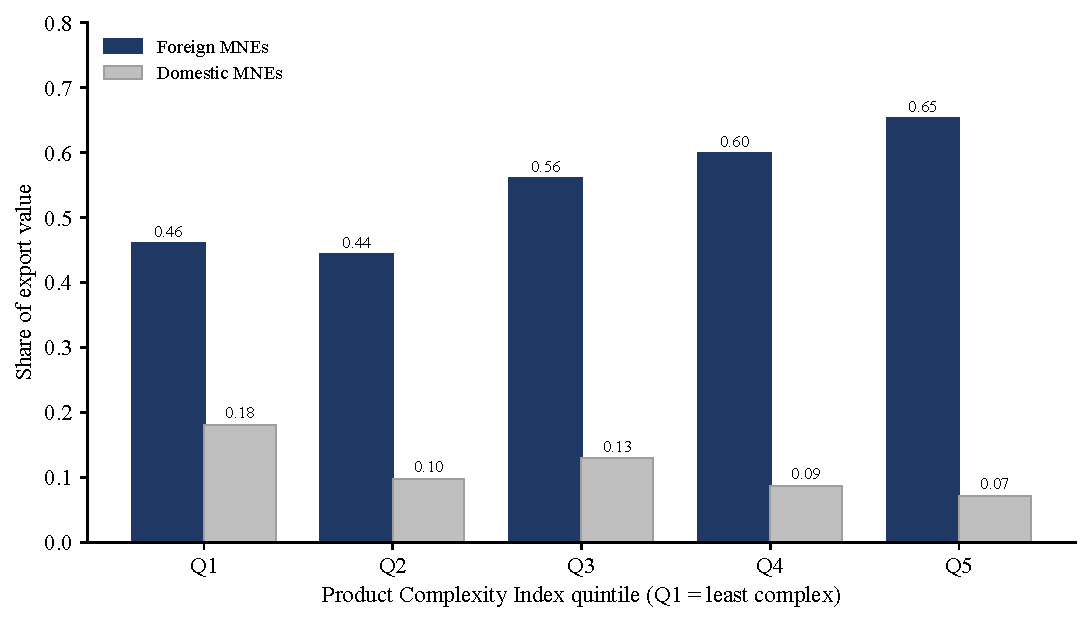
\includegraphics[width=\linewidth,height=0.38\textheight,keepaspectratio]{figures/all/fig_wp0_fig2_pci.pdf}%
  \end{minipage}\\[8pt]%
  \begin{minipage}[t]{0.72\textwidth}\centering\textbf{Panel B. Lall (2000) technology class}\\[2pt]%
  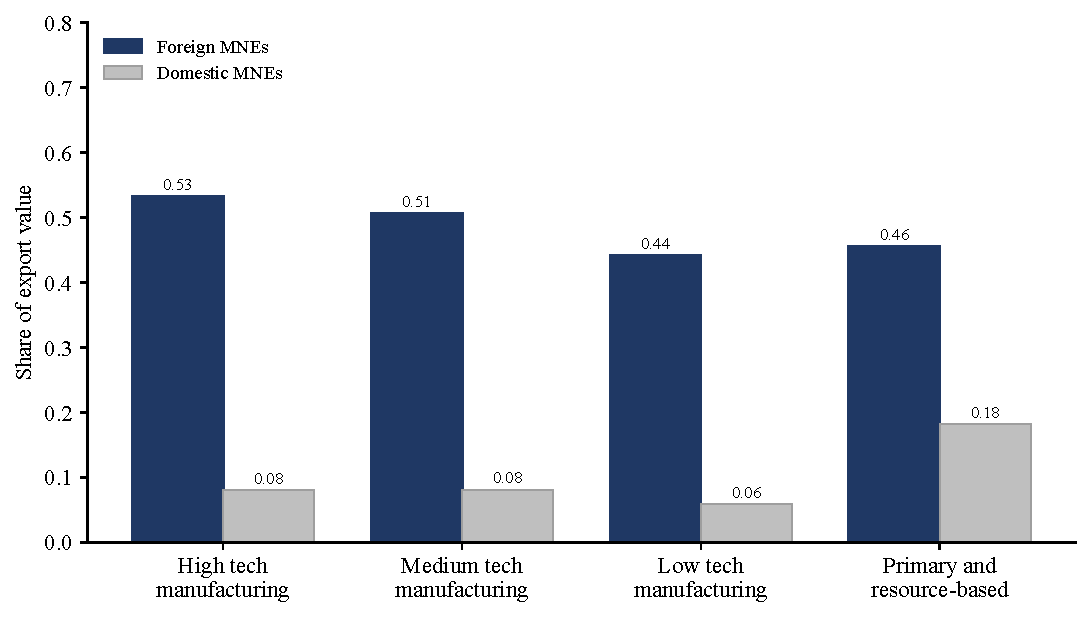
\includegraphics[width=\linewidth,height=0.38\textheight,keepaspectratio]{figures/all/fig_wp0_fig3_lall.pdf}%
  \end{minipage}%
  \caption{Multinational Share of Export Value, by Product Sophistication}%
  \label{fig:p_f2f3}%
  \par\vspace{2pt}%
  \parbox{0.92\textwidth}{\footnotesize %
  \textit{Notes:} Shares of export value, all available years pooled. Panel A: Quintiles of the Hausmann--Hidalgo Product Complexity Index across HS6 products (Q1 = least complex). Panel B: Lall (2000) technology classes: primary and resource-based products, and low-, medium- and high-technology manufactures.\\[3pt]%
  \textit{Source:} Authors' calculations based on customs data matched to Orbis and Dun \& Bradstreet.}%
  \end{figure}
% ---- Table: Multinational Share of Export Value, by Rauch Product Class
\begin{table}[H]\centering\small%
  \caption{Multinational Share of Export Value, by Rauch Product Class}%
  \label{tab:p_rauch}%
  \adjustbox{max width=\textwidth, max totalheight=0.8\textheight}{\begin{tabular}{lcccrr}
\toprule
Rauch (1999) class & Foreign & Domestic & All MNEs & HS6 products & Value (US\$bn/yr) \\
\midrule
Differentiated & 0.563 & 0.058 & 0.621 & 2,712 & 44.3 \\
Reference-priced & 0.549 & 0.082 & 0.631 & 1,636 & 63.7 \\
Homogeneous (exchange) & 0.343 & 0.228 & 0.571 & 319 & 97.6 \\
\bottomrule
\end{tabular}
}%
  \par\vspace{3pt}%
  \begin{minipage}{0.95\textwidth}\footnotesize %
  \textit{Notes:} Shares of export value, all available years pooled. Rauch (1999) conservative classification: homogeneous goods are traded on organized exchanges, reference-priced goods have a price quoted in trade publications, and differentiated goods have neither. Values are annual averages in US\$ billion.\\[3pt]%
  \textit{Source:} Authors' calculations based on customs data matched to Orbis and Dun \& Bradstreet.%
  \end{minipage}%
  \end{table}
% ---- Figure: Multinational Share of Export Value, by Rauch Product Class
\begin{figure}[H]\centering%
  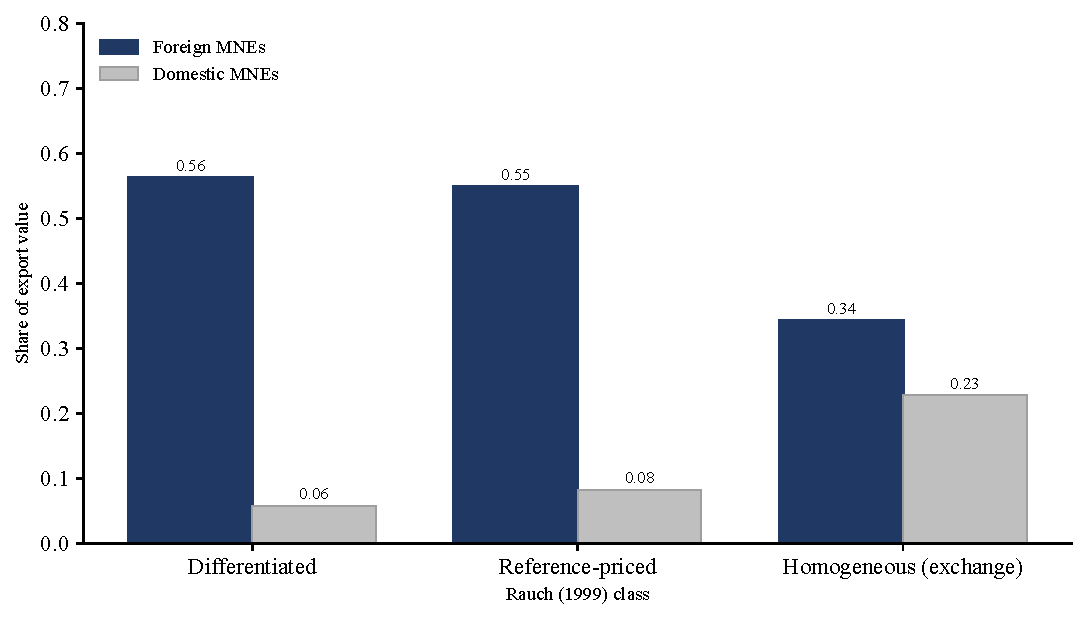
\includegraphics[width=0.7\textwidth,height=0.8\textheight,keepaspectratio]{figures/all/fig_wp1b_rauch.pdf}%
  \caption{Multinational Share of Export Value, by Rauch Product Class}%
  \label{fig:p_rauch_fig}%
  \par\vspace{2pt}%
  \parbox{0.92\textwidth}{\footnotesize %
  \textit{Notes:} Shares of export value, all available years pooled. Rauch (1999) conservative classification: homogeneous goods are traded on organized exchanges, reference-priced goods have a price quoted in trade publications, and differentiated goods have neither.\\[3pt]%
  \textit{Source:} Authors' calculations based on customs data matched to Orbis and Dun \& Bradstreet.}%
  \end{figure}
% ---- Table: Multinational Share of Export Value, by End Use
\begin{table}[H]\centering\small%
  \caption{Multinational Share of Export Value, by End Use}%
  \label{tab:p_bec}%
  \adjustbox{max width=\textwidth, max totalheight=0.8\textheight}{\begin{tabular}{lcccrr}
\toprule
BEC end use & Foreign & Domestic & All MNEs & HS6 products & Value (US\$bn/yr) \\
\midrule
Intermediate & 0.476 & 0.155 & 0.631 & 3,090 & 155.0 \\
Consumption & 0.438 & 0.082 & 0.520 & 1,201 & 46.1 \\
Capital & 0.647 & 0.056 & 0.703 & 659 & 9.3 \\
\bottomrule
\end{tabular}
}%
  \par\vspace{3pt}%
  \begin{minipage}{0.95\textwidth}\footnotesize %
  \textit{Notes:} Shares of export value, all available years pooled. End use from BEC Rev.\,4; HS6 products without a BEC correspondence are excluded. Values are annual averages in US\$ billion.\\[3pt]%
  \textit{Source:} Authors' calculations based on customs data matched to Orbis and Dun \& Bradstreet.%
  \end{minipage}%
  \end{table}
% ---- Table: Product Sophistication and Multinational Shares
\begin{table}[H]\centering\footnotesize%
  \caption{Product Sophistication and Multinational Shares}%
  \label{tab:p_ladder}%
  \adjustbox{max width=\textwidth, max totalheight=0.8\textheight}{\begin{tabular}{lcccccc} \hline
 & \multicolumn{2}{c}{PCI} & \multicolumn{2}{c}{Lall} & \multicolumn{2}{c}{Rauch} \\
 & (1) & (2) & (3) & (4) & (5) & (6) \\ \hline
\multicolumn{7}{l}{\textit{Panel A. Dependent variable: share of all MNEs}} \\
Complexity (PCI) & -0.0004 & 0.0052 &  &  &  &  \\
 & (0.0050) & (0.0045) &  &  &  &  \\
Lall: high tech (vs primary and resource-based) &  &  & -0.0288** & -0.0347** &  &  \\
 &  &  & (0.0142) & (0.0142) &  &  \\
Lall: medium tech &  &  & -0.0256*** & -0.0111 &  &  \\
 &  &  & (0.0081) & (0.0074) &  &  \\
Lall: low tech &  &  & -0.0801*** & -0.0797*** &  &  \\
 &  &  & (0.0165) & (0.0171) &  &  \\
Rauch: differentiated (vs homogeneous) &  &  &  &  & 0.0819*** & 0.0880*** \\
 &  &  &  &  & (0.0112) & (0.0104) \\
Rauch: reference-priced &  &  &  &  & 0.1038*** & 0.1132*** \\
 &  &  &  &  & (0.0103) & (0.0104) \\
Observations & 1,671,802 & 1,670,186 & 1,788,929 & 1,787,370 & 1,667,472 & 1,665,924 \\
\midrule
\multicolumn{7}{l}{\textit{Panel B. Dependent variable: share of foreign MNEs}} \\
Complexity (PCI) & 0.0385*** & 0.0280*** &  &  &  &  \\
 & (0.0052) & (0.0050) &  &  &  &  \\
Lall: high tech (vs primary and resource-based) &  &  & 0.0330** & 0.0140 &  &  \\
 &  &  & (0.0135) & (0.0129) &  &  \\
Lall: medium tech &  &  & 0.0400*** & 0.0517*** &  &  \\
 &  &  & (0.0080) & (0.0071) &  &  \\
Lall: low tech &  &  & -0.0000 & -0.0050 &  &  \\
 &  &  & (0.0118) & (0.0087) &  &  \\
Rauch: differentiated (vs homogeneous) &  &  &  &  & 0.2088*** & 0.1914*** \\
 &  &  &  &  & (0.0082) & (0.0079) \\
Rauch: reference-priced &  &  &  &  & 0.1783*** & 0.1659*** \\
 &  &  &  &  & (0.0099) & (0.0099) \\
Observations & 1,671,802 & 1,670,186 & 1,788,929 & 1,787,370 & 1,667,472 & 1,665,924 \\
\midrule
\multicolumn{7}{l}{\textit{Panel C. Dependent variable: share of domestic MNEs}} \\
Complexity (PCI) & -0.0389*** & -0.0227*** &  &  &  &  \\
 & (0.0058) & (0.0045) &  &  &  &  \\
Lall: high tech (vs primary and resource-based) &  &  & -0.0618*** & -0.0487*** &  &  \\
 &  &  & (0.0143) & (0.0137) &  &  \\
Lall: medium tech &  &  & -0.0657*** & -0.0628*** &  &  \\
 &  &  & (0.0087) & (0.0075) &  &  \\
Lall: low tech &  &  & -0.0801*** & -0.0747*** &  &  \\
 &  &  & (0.0148) & (0.0155) &  &  \\
Rauch: differentiated (vs homogeneous) &  &  &  &  & -0.1270*** & -0.1034*** \\
 &  &  &  &  & (0.0101) & (0.0084) \\
Rauch: reference-priced &  &  &  &  & -0.0745*** & -0.0527*** \\
 &  &  &  &  & (0.0086) & (0.0075) \\
Observations & 1,671,802 & 1,670,186 & 1,788,929 & 1,787,370 & 1,667,472 & 1,665,924 \\
\hline
Origin $\times$ year and destination $\times$ year FE & $\checkmark$ &  & $\checkmark$ &  & $\checkmark$ &  \\
Origin $\times$ dest.\ $\times$ year FE &  & $\checkmark$ &  & $\checkmark$ &  & $\checkmark$ \\
\hline
\end{tabular}
}%
  \par\vspace{3pt}%
  \begin{minipage}{0.95\textwidth}\footnotesize %
  \textit{Notes:} Observations are origin--destination--HS6--year cells. Dependent variable: share of the cell's export value shipped by each type of MNE. Omitted categories: primary and resource-based products (Lall) and homogeneous products (Rauch). Robust standard errors in parentheses. *** $p<0.01$, ** $p<0.05$, * $p<0.1$.\\[3pt]%
  \textit{Source:} Authors' calculations based on customs data matched to Orbis and Dun \& Bradstreet.%
  \end{minipage}%
  \end{table}
% ---- Figure: Manufacturing: Multinational Share of Export Value, by Rauch Product Class
\begin{figure}[H]\centering%
  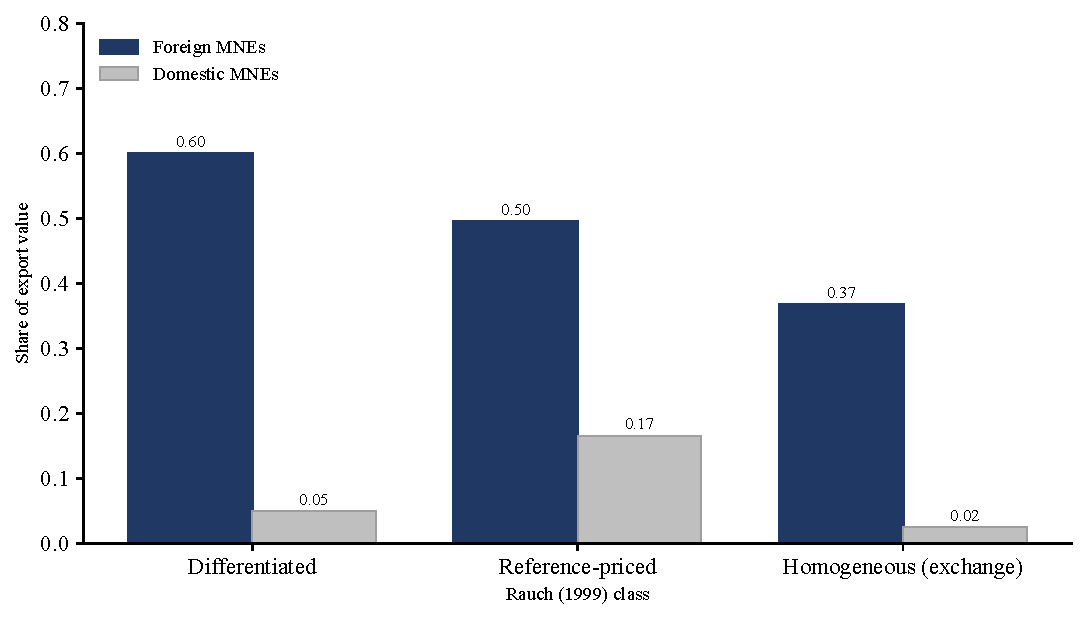
\includegraphics[width=0.7\textwidth,height=0.8\textheight,keepaspectratio]{figures/manufacturing/fig_wp1b_rauch.pdf}%
  \caption{Manufacturing: Multinational Share of Export Value, by Rauch Product Class}%
  \label{fig:p_rauch_manuf}%
  \par\vspace{2pt}%
  \parbox{0.92\textwidth}{\footnotesize %
  \textit{Notes:} Shares of manufacturing export value (HS 28--97 excluding 71), all available years pooled. Rauch (1999) conservative classification: homogeneous goods are traded on organized exchanges, reference-priced goods have a price quoted in trade publications, and differentiated goods have neither.\\[3pt]%
  \textit{Source:} Authors' calculations based on customs data matched to Orbis and Dun \& Bradstreet.}%
  \end{figure}

\subsection{Fact 3: Multinationals from a Small Set of Countries Dominate Exports}
Figure~\ref{fig:p_f4} ranks parent countries by their share of foreign-affiliate exports. The
United States (23 percent), the United Kingdom (19 percent) and Canada (8 percent) account for
half, and the ten largest parent countries for more than three quarters.
Table~\ref{tab:p_pxp} shows where the affiliates of each of the ten largest parent countries sell;
its diagonal is the share shipped to the parent's own country. The share is 22.3 percent for US
groups, 19.5 percent for Canadian groups and 18.6 percent for Brazilian groups, but less than 3
percent for British, Dutch or Swiss groups. Figure~\ref{fig:p_dest} shows the same pattern from the
side of the main destination markets.

% ---- Figure: Foreign-Multinational Exports, by Parent Country
\begin{figure}[H]\centering%
  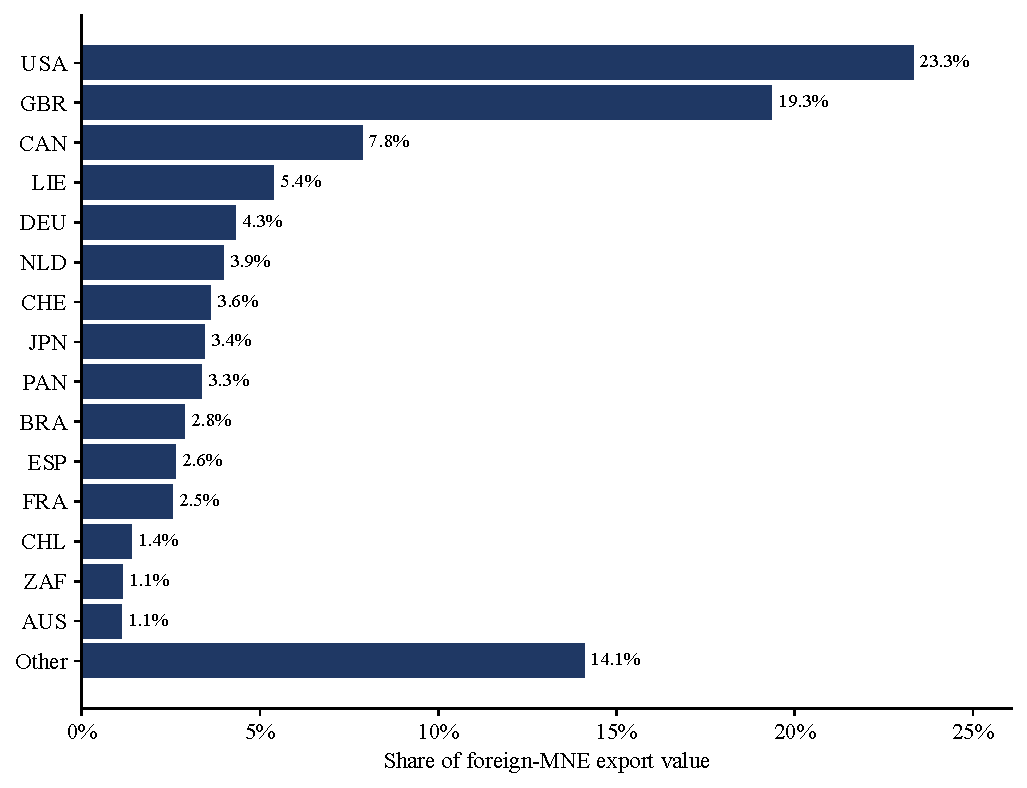
\includegraphics[width=0.78\textwidth,height=0.8\textheight,keepaspectratio]{figures/all/fig_wp1a_parent_share.pdf}%
  \caption{Foreign-Multinational Exports, by Parent Country}%
  \label{fig:p_f4}%
  \par\vspace{2pt}%
  \parbox{0.92\textwidth}{\footnotesize %
  \textit{Notes:} Percent of foreign-MNE export value, by country of the ultimate parent.\\[3pt]%
  \textit{Source:} Authors' calculations based on customs data matched to Orbis and Dun \& Bradstreet.}%
  \end{figure}
% ---- Table: Foreign-Multinational Exports to the Parent Countries, by Parent Country
\begin{table}[H]\centering\small%
  \caption{Foreign-Multinational Exports to the Parent Countries, by Parent Country}%
  \label{tab:p_pxp}%
  \adjustbox{max width=\textwidth, max totalheight=0.8\textheight}{\begin{tabular}{lrrrrrrrrrrrr}
\toprule
Parent / Destination & USA & GBR & CAN & LIE & DEU & NLD & CHE & JPN & PAN & BRA & Other destinations & Total \\
\midrule
USA & 22.3 & 1.0 & 0.5 & 0.0 & 0.6 & 3.5 & 1.7 & 3.8 & 2.7 & 7.8 & 56.2 & 100.0 \\
GBR & 5.6 & 0.6 & 3.3 & 0.0 & 3.6 & 3.2 & 0.6 & 7.1 & 0.2 & 3.9 & 71.8 & 100.0 \\
CAN & 6.6 & 2.6 & 19.5 & 0.0 & 3.5 & 0.9 & 12.9 & 5.3 & 2.6 & 4.2 & 41.8 & 100.0 \\
LIE & 3.7 & 0.4 & 0.0 & 0.0 & 0.9 & 1.8 & 0.2 & 18.7 & 0.1 & 3.7 & 70.5 & 100.0 \\
DEU & 14.8 & 0.3 & 1.1 & 0.0 & 8.3 & 1.0 & 0.0 & 1.1 & 0.8 & 31.9 & 40.6 & 100.0 \\
NLD & 3.8 & 0.5 & 0.2 & 0.0 & 0.4 & 2.2 & 0.0 & 0.4 & 0.4 & 26.9 & 65.2 & 100.0 \\
CHE & 5.0 & 1.0 & 0.4 & 0.0 & 0.7 & 2.0 & 0.3 & 0.5 & 1.7 & 6.8 & 81.6 & 100.0 \\
JPN & 8.7 & 0.3 & 0.5 & 0.0 & 0.2 & 0.9 & 0.0 & 8.9 & 1.0 & 45.0 & 34.5 & 100.0 \\
PAN & 9.5 & 0.8 & 0.6 & 0.0 & 1.7 & 2.0 & 0.2 & 1.8 & 1.4 & 1.2 & 80.7 & 100.0 \\
BRA & 14.1 & 0.5 & 0.6 & 0.0 & 2.3 & 2.1 & 2.2 & 1.6 & 0.6 & 18.6 & 57.4 & 100.0 \\
Other parents & 19.5 & 0.9 & 1.6 & 0.0 & 2.2 & 2.1 & 1.2 & 2.2 & 1.7 & 11.7 & 56.8 & 100.0 \\
\bottomrule
\end{tabular}
}%
  \par\vspace{3pt}%
  \begin{minipage}{0.95\textwidth}\footnotesize %
  \textit{Notes:} Percent of each parent country's exports, by destination (rows add to 100). Destinations are the ten largest parent countries; the diagonal is the share shipped to the parent's own country.\\[3pt]%
  \textit{Source:} Authors' calculations based on customs data matched to Orbis and Dun \& Bradstreet.%
  \end{minipage}%
  \end{table}
% ---- Figure: Ownership of Exports to the Main Destination Markets
\begin{figure}[H]\centering%
  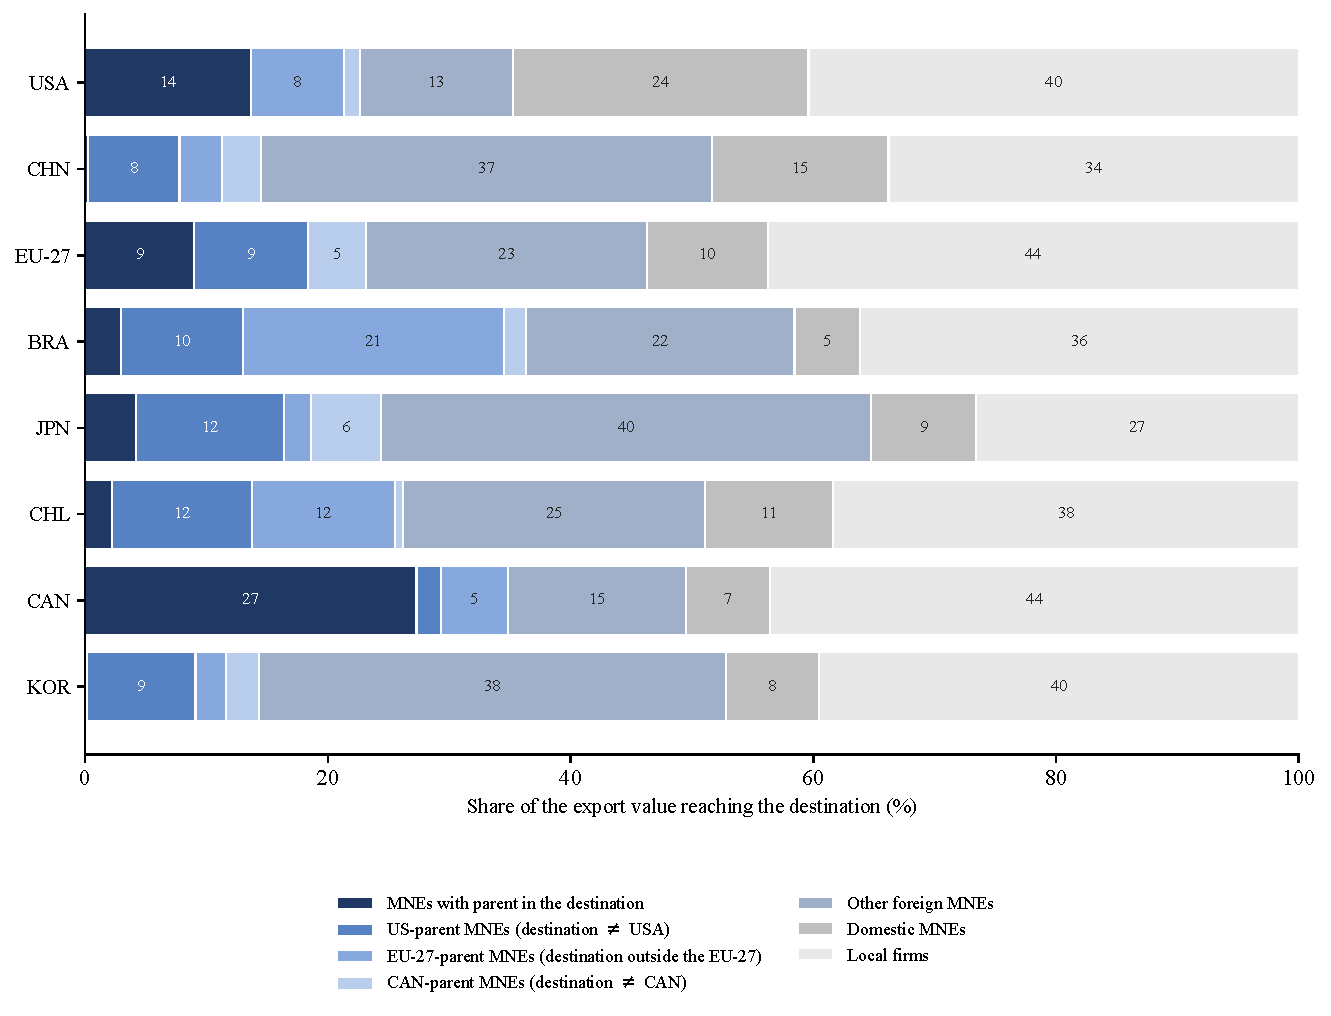
\includegraphics[width=1.0\textwidth,height=0.8\textheight,keepaspectratio]{figures/all/fig_wp3_dest_carriers.pdf}%
  \caption{Ownership of Exports to the Main Destination Markets}%
  \label{fig:p_dest}%
  \par\vspace{2pt}%
  \parbox{0.92\textwidth}{\footnotesize %
  \textit{Notes:} Percent of the export value reaching each destination, by type of exporter. The first segment is exports by MNEs whose parent is located in that destination. EU-27 member states are pooled.\\[3pt]%
  \textit{Source:} Authors' calculations based on customs data matched to Orbis and Dun \& Bradstreet.}%
  \end{figure}

\subsection{Fact 4: A Small Set of Large Multinational Groups Accounts for Most Exports}
Figure~\ref{fig:p_f5} groups parents by the number of affiliates their group has worldwide. Almost
half of the parents have a single affiliate, but the 9 percent with more than 100 affiliates
account for 56 percent of foreign-affiliate exports.

% ---- Figure: Foreign-Multinational Exports and Number of Parents, by Size of the Group's Global Network
\begin{figure}[H]\centering%
  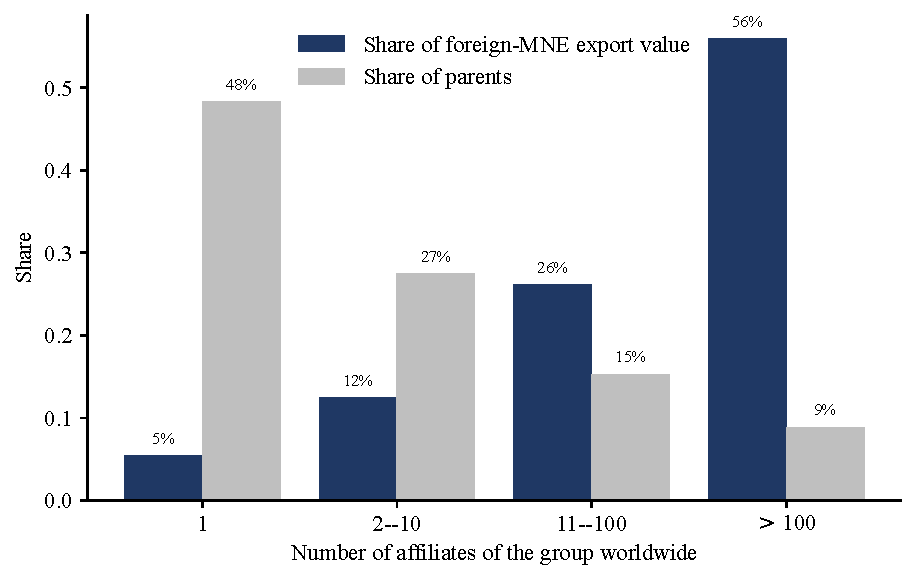
\includegraphics[width=0.7\textwidth,height=0.8\textheight,keepaspectratio]{figures/all/fig_wp0_fig5_network.pdf}%
  \caption{Foreign-Multinational Exports and Number of Parents, by Size of the Group's Global Network}%
  \label{fig:p_f5}%
  \par\vspace{2pt}%
  \parbox{0.92\textwidth}{\footnotesize %
  \textit{Notes:} Shares of foreign-MNE export value and of parents, by the number of affiliates the group has worldwide.\\[3pt]%
  \textit{Source:} Authors' calculations based on customs data matched to Orbis and Dun \& Bradstreet.}%
  \end{figure}

\subsection{Fact 5: Multinational Presence Is Associated with Higher Exports}
Table~\ref{tab:p_t1} relates the exports of an origin--destination--product--year cell to the
number of multinationals exporting in it (intensive margin) and to whether any does (extensive
margin). Both relationships are positive and large, also for the exports of the local firms in the
same cell (Panel~B). Table~\ref{tab:p_f5counts} splits the intensive margin by type of
multinational. The coefficient is 1.21 for foreign affiliates and 0.44 for domestic ones in
Panel~A, and 1.13 and 0.47 in Panel~B. On the extensive margin the two coefficients are almost
equal (Table~\ref{tab:a_ext}).

% ---- Table: Multinational Presence and Exports
\begin{table}[H]\centering\small%
  \caption{Multinational Presence and Exports}%
  \label{tab:p_t1}%
  \adjustbox{max width=\textwidth, max totalheight=0.8\textheight}{\begin{tabular}{lcccccc} \hline
 & \multicolumn{3}{c}{Intensive: $\ln$(\# MNE firms)} & \multicolumn{3}{c}{Extensive: any MNE present} \\
 & (1) & (2) & (3) & (1) & (2) & (3) \\ \hline
\multicolumn{7}{l}{\textit{Panel A. Dependent variable: $\ln$ exports, all firms}} \\
$\ln$(\# MNE firms) & 2.0823*** & 2.0685*** & 0.9414*** &  &  &  \\
 & (0.0363) & (0.0368) & (0.0206) &  &  &  \\
Any MNE present &  &  &  & 1.4622*** & 1.4591*** & 0.6818*** \\
 &  &  &  & (0.0394) & (0.0388) & (0.0165) \\
\midrule
\multicolumn{7}{l}{\textit{Panel B. Dependent variable: $\ln$ exports, non-MNE firms}} \\
$\ln$(\# MNE firms) & 1.3536*** & 1.3406*** & 0.2389*** &  &  &  \\
 & (0.0318) & (0.0319) & (0.0178) &  &  &  \\
Any MNE present &  &  &  & 1.4168*** & 1.3996*** & 0.1311*** \\
 &  &  &  & (0.0371) & (0.0367) & (0.0102) \\
\hline
Origin FE & $\checkmark$ &  &  & $\checkmark$ &  &  \\
Destination FE & $\checkmark$ &  &  & $\checkmark$ &  &  \\
Product FE & $\checkmark$ & $\checkmark$ &  & $\checkmark$ & $\checkmark$ &  \\
Year FE & $\checkmark$ &  &  & $\checkmark$ &  &  \\
Origin $\times$ year FE &  & $\checkmark$ &  &  & $\checkmark$ &  \\
Destination $\times$ year FE &  & $\checkmark$ &  &  & $\checkmark$ &  \\
Origin $\times$ dest.\ $\times$ product FE &  &  & $\checkmark$ &  &  & $\checkmark$ \\
Origin $\times$ dest.\ $\times$ year FE &  &  & $\checkmark$ &  &  & $\checkmark$ \\
Observations (Panel A) & 1,008,472 & 1,008,185 & 883,545 & 1,829,852 & 1,829,626 & 1,633,319 \\
Observations (Panel B) & 475,856 & 475,514 & 429,882 & 1,297,322 & 1,297,111 & 1,137,550 \\
\hline
\end{tabular}
}%
  \par\vspace{3pt}%
  \begin{minipage}{0.95\textwidth}\footnotesize %
  \textit{Notes:} Observations are origin--destination--HS6--year cells. Dependent variable: $\ln$ exports of the cell (Panel A) and of the non-MNE firms in the cell (Panel B). Intensive margin: $\ln$ number of MNEs, cells with at least one MNE. Extensive margin: indicator for at least one MNE. Standard errors clustered by origin--destination pair in parentheses. *** $p<0.01$, ** $p<0.05$, * $p<0.1$.\\[3pt]%
  \textit{Source:} Authors' calculations based on customs data matched to Orbis and Dun \& Bradstreet.%
  \end{minipage}%
  \end{table}
% ---- Table: Multinational Presence and Exports: Intensive Margin, by Type of Multinational
\begin{table}[H]\centering\small%
  \caption{Multinational Presence and Exports: Intensive Margin, by Type of Multinational}%
  \label{tab:p_f5counts}%
  \adjustbox{max width=\textwidth, max totalheight=0.8\textheight}{\begin{tabular}{lcccccc} \hline
 & \multicolumn{2}{c}{All MNEs} & \multicolumn{2}{c}{Foreign / domestic} & \multicolumn{2}{c}{Foreign by destination, domestic} \\
 & (1) & (2) & (3) & (4) & (5) & (6) \\ \hline
\multicolumn{7}{l}{\textit{Panel A. Dependent variable: $\ln$ exports, all firms}} \\
$\ln$(\# MNE firms) & 2.0685*** & 0.9414*** &  &  &  &  \\
 & (0.0368) & (0.0206) &  &  &  &  \\
$\ln$(\# foreign MNEs) &  &  & 1.2129*** & 0.4506*** &  &  \\
 &  &  & (0.0285) & (0.0124) &  &  \\
$\ln$(\# foreign MNEs, parent-country destination) &  &  &  &  & 0.3970*** & 0.1448*** \\
 &  &  &  &  & (0.0856) & (0.0370) \\
$\ln$(\# foreign MNEs, other destinations) &  &  &  &  & 0.9465*** & 0.3133*** \\
 &  &  &  &  & (0.0536) & (0.0382) \\
$\ln$(\# domestic MNEs) &  &  & 0.4382*** & 0.2214*** & 0.3770*** & 0.1555*** \\
 &  &  & (0.0259) & (0.0151) & (0.0514) & (0.0315) \\
\midrule
\multicolumn{7}{l}{\textit{Panel B. Dependent variable: $\ln$ exports, non-MNE firms}} \\
$\ln$(\# MNE firms) & 1.3406*** & 0.2389*** &  &  &  &  \\
 & (0.0319) & (0.0178) &  &  &  &  \\
$\ln$(\# foreign MNEs) &  &  & 1.1331*** & 0.2413*** &  &  \\
 &  &  & (0.0375) & (0.0217) &  &  \\
$\ln$(\# foreign MNEs, parent-country destination) &  &  &  &  & 0.2934*** & 0.1945*** \\
 &  &  &  &  & (0.0882) & (0.0527) \\
$\ln$(\# foreign MNEs, other destinations) &  &  &  &  & 1.0330*** & 0.1951*** \\
 &  &  &  &  & (0.0607) & (0.0648) \\
$\ln$(\# domestic MNEs) &  &  & 0.4707*** & 0.1250*** & 0.4142*** & 0.0946* \\
 &  &  & (0.0341) & (0.0218) & (0.0633) & (0.0552) \\
\hline
Product FE & $\checkmark$ &  & $\checkmark$ &  & $\checkmark$ &  \\
Origin $\times$ year FE & $\checkmark$ &  & $\checkmark$ &  & $\checkmark$ &  \\
Destination $\times$ year FE & $\checkmark$ &  & $\checkmark$ &  & $\checkmark$ &  \\
Origin $\times$ dest.\ $\times$ product FE &  & $\checkmark$ &  & $\checkmark$ &  & $\checkmark$ \\
Origin $\times$ dest.\ $\times$ year FE &  & $\checkmark$ &  & $\checkmark$ &  & $\checkmark$ \\
Observations (Panel A) & 1,008,185 & 883,545 & 113,422 & 98,223 & 9,197 & 7,524 \\
Observations (Panel B) & 475,514 & 429,882 & 93,010 & 81,563 & 8,780 & 7,255 \\
\hline
\end{tabular}
}%
  \par\vspace{3pt}%
  \begin{minipage}{0.95\textwidth}\footnotesize %
  \textit{Notes:} Observations are origin--destination--HS6--year cells. Dependent variable: $\ln$ exports of the cell (Panel A) and of the non-MNE firms in the cell (Panel B). Regressors: $\ln$ number of MNEs of each type. Columns (5)--(6) split foreign MNEs by whether the destination is the parent's country. Standard errors clustered by origin--destination pair in parentheses. *** $p<0.01$, ** $p<0.05$, * $p<0.1$.\\[3pt]%
  \textit{Source:} Authors' calculations based on customs data matched to Orbis and Dun \& Bradstreet.%
  \end{minipage}%
  \end{table}

\subsection{Fact 6: Distance Is a Weaker Barrier for Multinationals}
Table~\ref{tab:p_t2} estimates how firm exports fall with distance. The elasticity is $-0.16$ for
local firms and about 0.05 smaller in absolute value for multinationals. Table~\ref{tab:p_dist}
shows that the difference is larger for foreign affiliates (0.049) than for domestic ones (0.032),
and largest for foreign affiliates exporting to their parent's country (0.064).

% ---- Table: Distance and Firm Exports: Multinationals by Presence at the Destination
\begin{table}[H]\centering\small%
  \caption{Distance and Firm Exports: Multinationals by Presence at the Destination}%
  \label{tab:p_t2}%
  \adjustbox{max width=\textwidth, max totalheight=0.8\textheight}{\begin{tabular}{lcccc} \hline
Dep.\ var.: $\ln$ exports & (1) & (2) & (3) & (4) \\ \hline
$\ln$ distance & -0.1639*** & -0.1848*** & -0.1632*** & -0.1838*** \\
 & (0.0454) & (0.0460) & (0.0452) & (0.0459) \\
$\ln$ distance $\times$ MNE & 0.0461*** & 0.0458*** &  &  \\
 & (0.0038) & (0.0038) &  &  \\
$\ln$ distance $\times$ MNE, present at destination &  &  & 0.0689*** & 0.0682*** \\
 &  &  & (0.0070) & (0.0070) \\
$\ln$ distance $\times$ MNE, not present at destination &  &  & 0.0393*** & 0.0391*** \\
 &  &  & (0.0032) & (0.0032) \\
\hline
Origin FE & $\checkmark$ &  & $\checkmark$ &  \\
Destination FE & $\checkmark$ &  & $\checkmark$ &  \\
Year FE & $\checkmark$ &  & $\checkmark$ &  \\
Origin $\times$ year FE &  & $\checkmark$ &  & $\checkmark$ \\
Destination $\times$ year FE &  & $\checkmark$ &  & $\checkmark$ \\
Product FE & $\checkmark$ & $\checkmark$ & $\checkmark$ & $\checkmark$ \\
\hline
Observations & 5,081,547 & 5,081,360 & 5,081,547 & 5,081,360 \\
\hline
\end{tabular}
}%
  \par\vspace{3pt}%
  \begin{minipage}{0.95\textwidth}\footnotesize %
  \textit{Notes:} Observations are firm--destination--HS6--year cells. Dependent variable: $\ln$ exports. Non-MNE firms are the omitted group. Present: the group has an affiliate in the destination or the destination is the parent's country. Standard errors clustered by origin--destination pair in parentheses. *** $p<0.01$, ** $p<0.05$, * $p<0.1$.\\[3pt]%
  \textit{Source:} Authors' calculations based on customs data matched to Orbis and Dun \& Bradstreet.%
  \end{minipage}%
  \end{table}
% ---- Table: Distance and Firm Exports: Foreign and Domestic Multinationals
\begin{table}[H]\centering\small%
  \caption{Distance and Firm Exports: Foreign and Domestic Multinationals}%
  \label{tab:p_dist}%
  \adjustbox{max width=\textwidth, max totalheight=0.8\textheight}{\begin{tabular}{lcccc} \hline
Dep.\ var.: $\ln$ exports & (1) & (2) & (3) & (4) \\ \hline
$\ln$ distance & -0.1645*** & -0.1853*** & -0.1644*** & -0.1851*** \\
 & (0.0454) & (0.0460) & (0.0454) & (0.0460) \\
$\ln$ distance $\times$ foreign MNE & 0.0487*** & 0.0483*** &  &  \\
 & (0.0041) & (0.0040) &  &  \\
$\ln$ distance $\times$ foreign MNE, parent-country destination &  &  & 0.0642*** & 0.0638*** \\
 &  &  & (0.0159) & (0.0161) \\
$\ln$ distance $\times$ foreign MNE, other destination &  &  & 0.0477*** & 0.0473*** \\
 &  &  & (0.0035) & (0.0035) \\
$\ln$ distance $\times$ domestic MNE & 0.0318*** & 0.0318*** & 0.0317*** & 0.0317*** \\
 & (0.0042) & (0.0042) & (0.0042) & (0.0042) \\
\hline
Origin FE & $\checkmark$ &  & $\checkmark$ &  \\
Destination FE & $\checkmark$ &  & $\checkmark$ &  \\
Year FE & $\checkmark$ &  & $\checkmark$ &  \\
Origin $\times$ year FE &  & $\checkmark$ &  & $\checkmark$ \\
Destination $\times$ year FE &  & $\checkmark$ &  & $\checkmark$ \\
Product FE & $\checkmark$ & $\checkmark$ & $\checkmark$ & $\checkmark$ \\
\hline
Observations & 5,081,547 & 5,081,360 & 5,081,547 & 5,081,360 \\
\hline
\end{tabular}
}%
  \par\vspace{3pt}%
  \begin{minipage}{0.95\textwidth}\footnotesize %
  \textit{Notes:} Observations are firm--destination--HS6--year cells. Dependent variable: $\ln$ exports. Non-MNE firms are the omitted group. Columns (3)--(4) split foreign MNEs by whether the destination is the parent's country. Standard errors clustered by origin--destination pair in parentheses. *** $p<0.01$, ** $p<0.05$, * $p<0.1$.\\[3pt]%
  \textit{Source:} Authors' calculations based on customs data matched to Orbis and Dun \& Bradstreet.%
  \end{minipage}%
  \end{table}

\section{Products}\label{sec:products}
Figure~\ref{fig:p_hs6} shows the twenty largest export products and who exports them. Crude
petroleum is mostly exported by domestic multinationals and copper concentrates by foreign ones.
Figure~\ref{fig:p_hs6_parent} splits the foreign share by parent country: British groups in copper
and coal, Canadian groups in gold, US groups in soybeans, maize and apparel, German groups in
trucks. Table~\ref{tab:p_sections} gives the same information by HS section, and
Tables~\ref{tab:a_agro_sitc} to~\ref{tab:a_mining_bec} in the appendix break down agriculture,
manufacturing and mining.

% ---- Figure: Ownership of the Twenty Largest Export Products
\begin{figure}[H]\centering%
  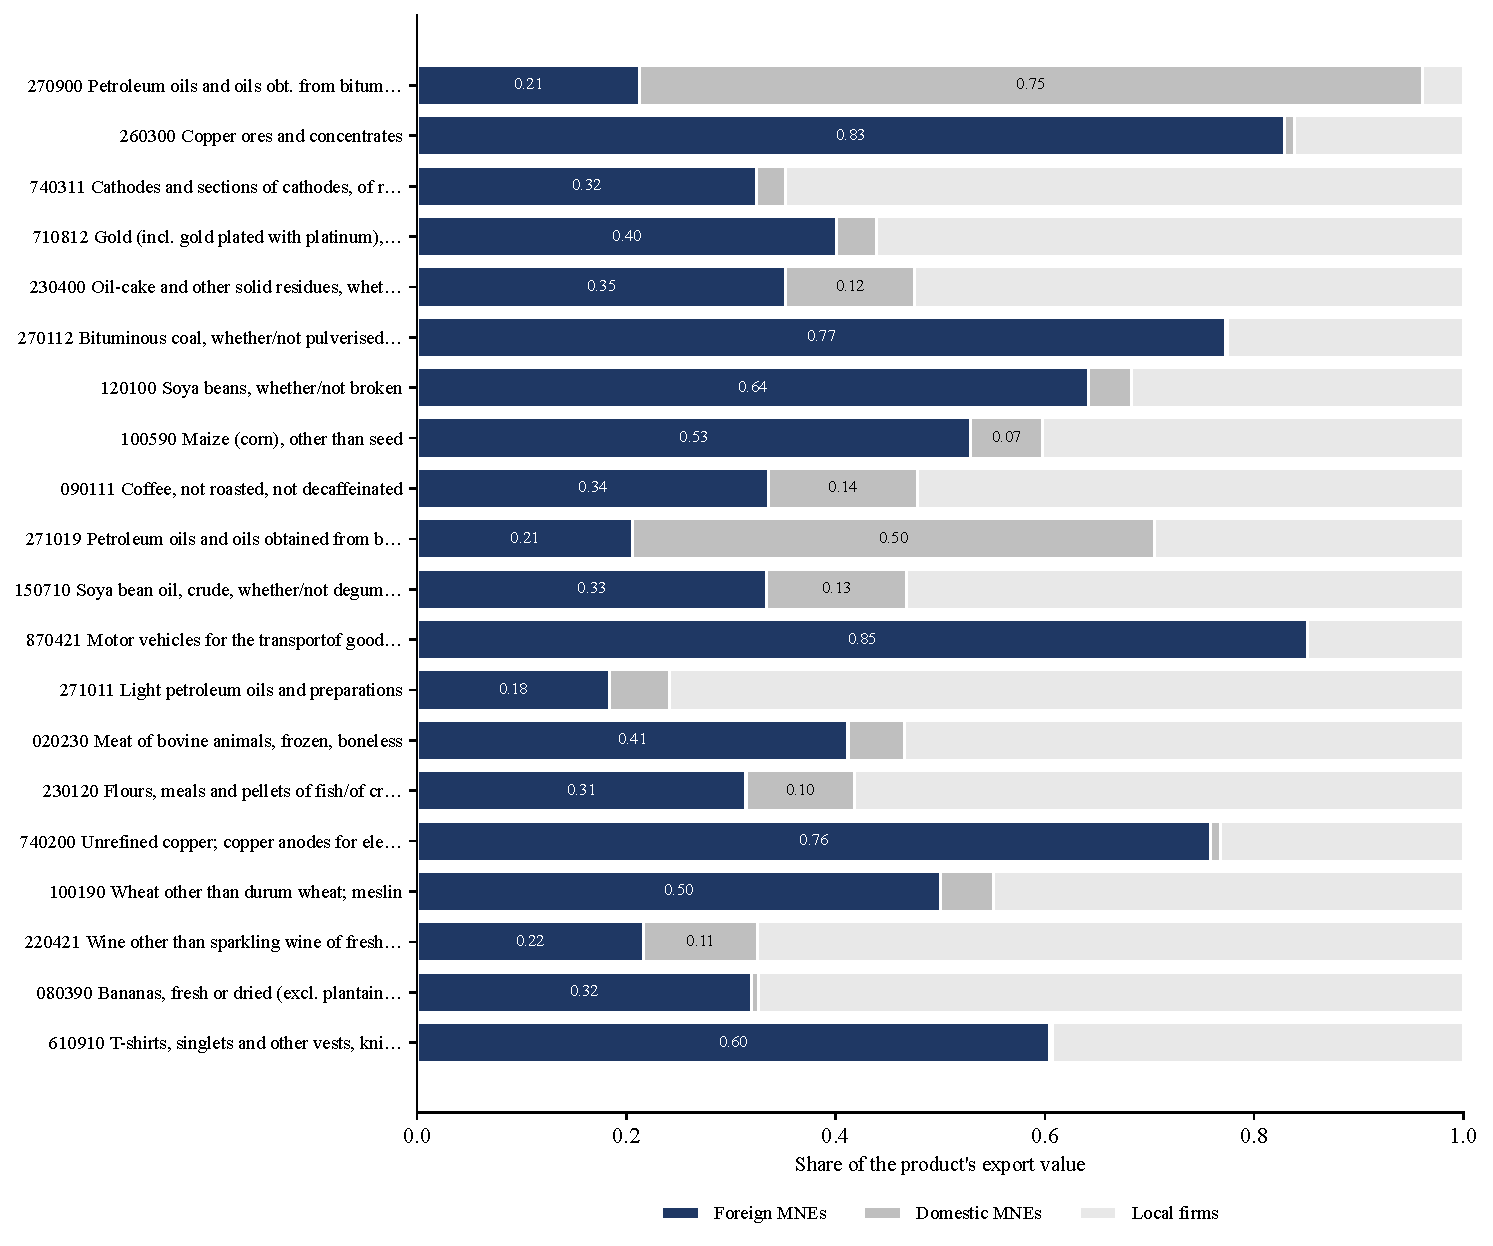
\includegraphics[width=1.0\textwidth,height=0.8\textheight,keepaspectratio]{figures/all/fig_wp1f_top20_hs6_stacked.pdf}%
  \caption{Ownership of the Twenty Largest Export Products}%
  \label{fig:p_hs6}%
  \par\vspace{2pt}%
  \parbox{0.92\textwidth}{\footnotesize %
  \textit{Notes:} Shares of each product's export value. Twenty largest HS6 products by export value.\\[3pt]%
  \textit{Source:} Authors' calculations based on customs data matched to Orbis and Dun \& Bradstreet.}%
  \end{figure}
% ---- Figure: Ownership of the Twenty Largest Export Products, by Parent Country
\begin{figure}[H]\centering%
  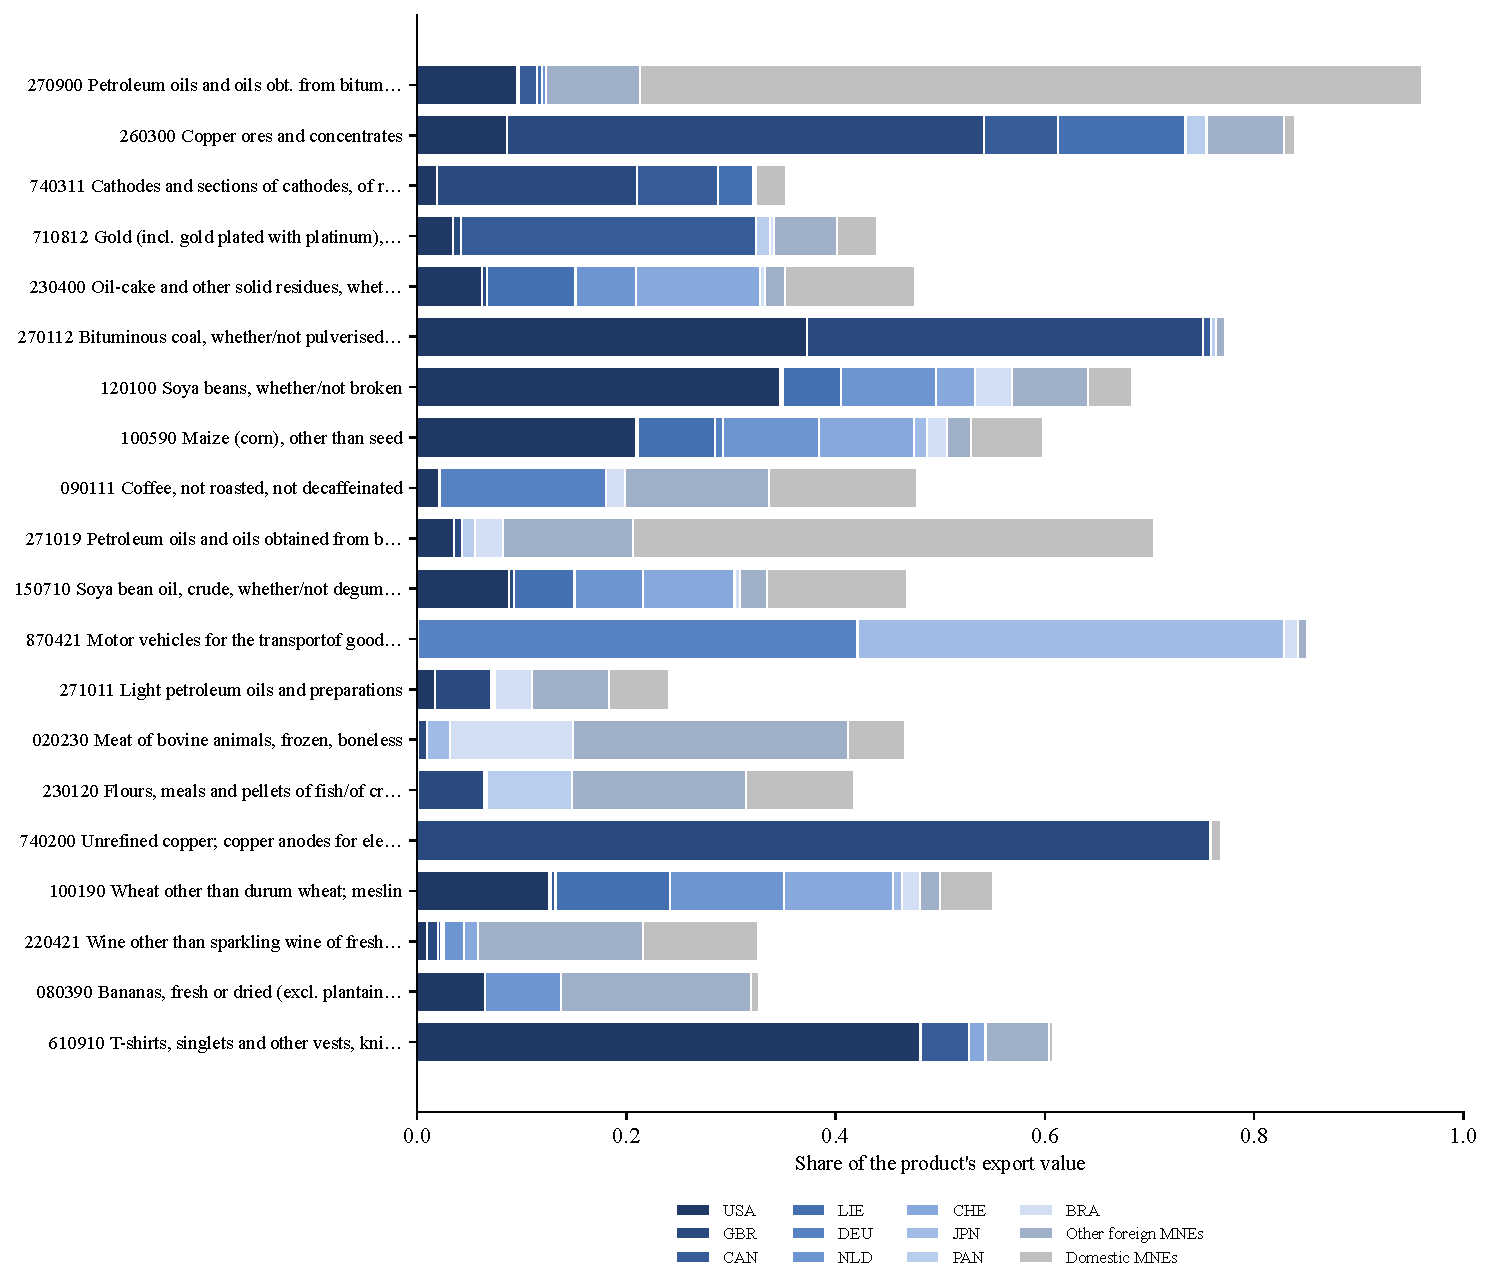
\includegraphics[width=1.0\textwidth,height=0.8\textheight,keepaspectratio]{figures/all/fig_wp1f_top20_hs6_by_parent.pdf}%
  \caption{Ownership of the Twenty Largest Export Products, by Parent Country}%
  \label{fig:p_hs6_parent}%
  \par\vspace{2pt}%
  \parbox{0.92\textwidth}{\footnotesize %
  \textit{Notes:} Shares of each product's export value. Foreign-MNE share split by country of the ultimate parent; the unfilled part of each bar is local firms.\\[3pt]%
  \textit{Source:} Authors' calculations based on customs data matched to Orbis and Dun \& Bradstreet.}%
  \end{figure}
% ---- Table: Exports and Multinational Shares, by HS Section
\begin{table}[H]\centering\footnotesize%
  \caption{Exports and Multinational Shares, by HS Section}%
  \label{tab:p_sections}%
  \adjustbox{max width=\textwidth, max totalheight=0.8\textheight}{\begin{tabular}{@{}p{7.2cm} r r r r l@{}}
\toprule
HS section & \$bn/yr & For. & Domestic & Local & Lead parent \\
\midrule
V Mineral products & 57.1 & 51 & 29 & 19 & GBR (0.42) \\
II Vegetable products & 33.5 & 42 & 7 & 51 & USA (0.33) \\
IV Prepared foodstuffs, beverages, tobacco & 25.9 & 37 & 10 & 53 & USA (0.21) \\
XV Base metals & 19.6 & 41 & 3 & 56 & GBR (0.44) \\
XIV Precious metals and stones & 15.3 & 41 & 4 & 56 & CAN (0.65) \\
I Live animals; animal products & 12.5 & 34 & 14 & 51 & SAU (0.19) \\
VI Chemicals & 11.6 & 49 & 14 & 37 & USA (0.25) \\
XVII Transport equipment & 9.7 & 78 & 4 & 18 & DEU (0.30) \\
XI Textiles and apparel & 6.9 & 49 & 3 & 48 & USA (0.62) \\
III Fats and oils & 6.9 & 31 & 10 & 59 & CHE (0.26) \\
XVI Machinery and electrical equipment & 6.2 & 63 & 4 & 33 & USA (0.41) \\
VII Plastics and rubber & 5.8 & 51 & 8 & 42 & USA (0.34) \\
X Pulp, paper & 3.4 & 54 & 28 & 18 & PAN (0.54) \\
XVIII Optical, precision instruments & 3.4 & 72 & 8 & 19 & USA (0.66) \\
IX Wood and articles & 1.9 & 27 & 34 & 39 & BHS (0.24) \\
VIII Hides, skins, leather & 1.6 & 40 & 12 & 49 & BGR (0.19) \\
XIII Stone, ceramics, glass & 0.9 & 49 & 4 & 46 & USA (0.32) \\
XX Miscellaneous manufactures & 0.9 & 53 & 7 & 40 & USA (0.48) \\
Unclassified & 0.5 & 49 & 29 & 23 & USA (0.39) \\
XII Footwear, headgear & 0.5 & 48 & 1 & 50 & USA (0.66) \\
XXI Works of art & 0.1 & 58 & 1 & 41 & BGR (0.94) \\
XIX Arms & 0.0 & 1 & 0 & 99 & CHE (0.82) \\
Special / unclassified (98-99) & 0.0 & 13 & 1 & 87 & USA (0.57) \\
\midrule
All sections & 224.5 & 46 & 14 & 40 & \\
\bottomrule
\end{tabular}
}%
  \par\vspace{3pt}%
  \begin{minipage}{0.95\textwidth}\footnotesize %
  \textit{Notes:} Foreign, domestic and local: percent of each section's export value. Leading parent: largest parent country and its share of the section's foreign-MNE exports. Values are annual averages in US\$ billion.\\[3pt]%
  \textit{Source:} Authors' calculations based on customs data matched to Orbis and Dun \& Bradstreet.%
  \end{minipage}%
  \end{table}

\section{Theoretical Framework}\label{sec:model}
\tbw{To be written. The model is developed in the companion theory paper.}


\section{Concluding Remarks}\label{sec:concl}
\tbw{To be written.}


\section*{References}%
\addcontentsline{toc}{section}{References}\label{sec:refs}
\tbw{To be completed.}
\begin{list}{}{\leftmargin=1.5em \itemindent=-1.5em \itemsep=2pt \topsep=4pt}
\item Hausmann, R. and Hidalgo, C., 2011. The Network Structure of Economic Output.
\emph{Journal of Economic Growth}, 16(4).
\item Lall, S., 2000. The Technological Structure and Performance of Developing Country
Manufactured Exports, 1985--98. \emph{Oxford Development Studies}, 28(3).
\item Rauch, J., 1999. Networks versus Markets in International Trade. \emph{Journal of
International Economics}, 48(1).
\item United Nations Statistics Division, 2022. \emph{Classification by Broad Economic
Categories}, Rev.\,4. New York.
\end{list}


\clearpage
\appendix
\setcounter{figure}{0}\renewcommand{\thefigure}{A.\arabic{figure}}
\setcounter{table}{0}\renewcommand{\thetable}{A.\arabic{table}}

\section{Additional Tables and Figures}\label{sec:app}

\subsection*{Fact 1}
% ---- Table: Multinational Share of Export Value, by Exporting Country
\begin{table}[H]\centering\small%
  \caption{Multinational Share of Export Value, by Exporting Country}%
  \label{tab:a_f1n}%
  \adjustbox{max width=\textwidth, max totalheight=0.8\textheight}{\begin{tabular}{lrrrr}
\toprule
Origin & Foreign & Domestic & All MNEs & Value (US\$bn/yr) \\
\midrule
COL & 0.353 & 0.391 & 0.744 & 44.0 \\
DOM & 0.684 & 0.013 & 0.697 & 8.6 \\
CRI & 0.597 & 0.036 & 0.633 & 10.5 \\
URY & 0.528 & 0.100 & 0.628 & 7.0 \\
PRY & 0.611 & 0.011 & 0.622 & 7.3 \\
CHL & 0.479 & 0.136 & 0.615 & 34.2 \\
ARG & 0.489 & 0.075 & 0.564 & 66.4 \\
SLV & 0.474 & 0.003 & 0.477 & 5.0 \\
PER & 0.442 & 0.023 & 0.466 & 41.4 \\
\midrule
All & 0.463 & 0.141 & 0.605 & 224.5 \\
\bottomrule
\end{tabular}
}%
  \par\vspace{3pt}%
  \begin{minipage}{0.95\textwidth}\footnotesize %
  \textit{Notes:} Shares of each country's export value, all available years pooled. Values are annual averages in US\$ billion.\\[3pt]%
  \textit{Source:} Authors' calculations based on customs data matched to Orbis and Dun \& Bradstreet.%
  \end{minipage}%
  \end{table}
% ---- Figure: Multinational Share of Export Value, by Exporting Country and Parent Country
\begin{figure}[H]\centering%
  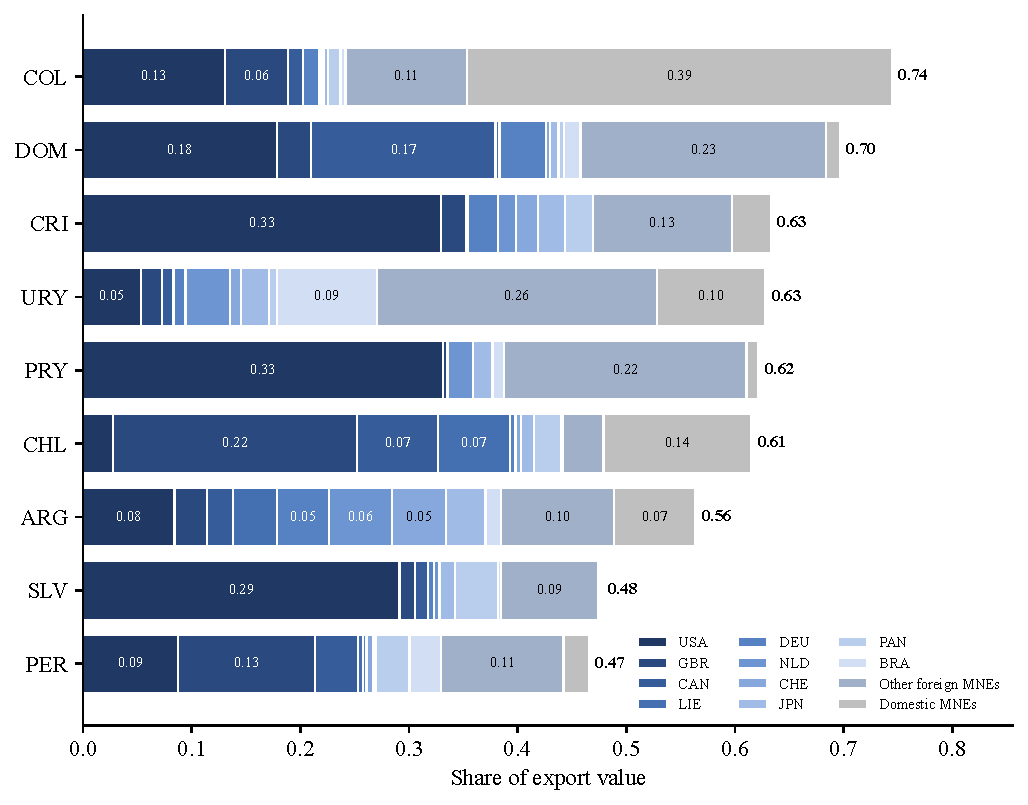
\includegraphics[width=0.92\textwidth,height=0.8\textheight,keepaspectratio]{figures/all/fig_wp1a_origin_by_parent.pdf}%
  \caption{Multinational Share of Export Value, by Exporting Country and Parent Country}%
  \label{fig:a_f1_parent}%
  \par\vspace{2pt}%
  \parbox{0.92\textwidth}{\footnotesize %
  \textit{Notes:} Shares of each country's export value. Foreign MNEs split by country of the ultimate parent; the ten largest parent countries are shown separately.\\[3pt]%
  \textit{Source:} Authors' calculations based on customs data matched to Orbis and Dun \& Bradstreet.}%
  \end{figure}
% ---- Table: Multinational Share of Export Value, by Exporting Country and Parent Country
\begin{table}[H]\centering\small%
  \caption{Multinational Share of Export Value, by Exporting Country and Parent Country}%
  \label{tab:a_f1pn}%
  \adjustbox{max width=\textwidth, max totalheight=0.8\textheight}{\begin{tabular}{lcccccccccccccc}
\toprule
Origin & USA & GBR & CAN & LIE & DEU & NLD & CHE & JPN & PAN & BRA & Other & Domestic & All MNEs & Value (US\$bn/yr) \\
\midrule
COL & 0.131 & 0.058 & 0.013 & 0.000 & 0.015 & 0.002 & 0.002 & 0.004 & 0.011 & 0.005 & 0.112 & 0.391 & 0.744 & 44.0 \\
DOM & 0.178 & 0.032 & 0.170 & 0.004 & 0.043 & 0.000 & 0.004 & 0.007 & 0.005 & 0.015 & 0.226 & 0.013 & 0.697 & 8.6 \\
CRI & 0.330 & 0.023 & 0.002 & 0.000 & 0.027 & 0.016 & 0.020 & 0.025 & 0.025 & 0.000 & 0.128 & 0.036 & 0.633 & 10.5 \\
URY & 0.053 & 0.020 & 0.010 & 0.000 & 0.011 & 0.041 & 0.010 & 0.026 & 0.008 & 0.091 & 0.258 & 0.100 & 0.628 & 7.0 \\
PRY & 0.331 & 0.004 & 0.000 & 0.000 & 0.000 & 0.023 & 0.000 & 0.017 & 0.001 & 0.010 & 0.223 & 0.011 & 0.622 & 7.3 \\
CHL & 0.028 & 0.225 & 0.074 & 0.066 & 0.005 & 0.000 & 0.005 & 0.012 & 0.025 & 0.001 & 0.037 & 0.136 & 0.615 & 34.2 \\
ARG & 0.084 & 0.030 & 0.024 & 0.041 & 0.047 & 0.058 & 0.050 & 0.036 & 0.001 & 0.014 & 0.104 & 0.075 & 0.564 & 66.4 \\
SLV & 0.291 & 0.015 & 0.012 & 0.000 & 0.006 & 0.005 & 0.000 & 0.014 & 0.040 & 0.003 & 0.090 & 0.003 & 0.477 & 5.0 \\
PER & 0.088 & 0.126 & 0.040 & 0.005 & 0.003 & 0.001 & 0.006 & 0.002 & 0.031 & 0.029 & 0.113 & 0.023 & 0.466 & 41.4 \\
\bottomrule
\end{tabular}
}%
  \par\vspace{3pt}%
  \begin{minipage}{0.95\textwidth}\footnotesize %
  \textit{Notes:} Shares of each country's export value. Other: all remaining foreign parents. Values are annual averages in US\$ billion.\\[3pt]%
  \textit{Source:} Authors' calculations based on customs data matched to Orbis and Dun \& Bradstreet.%
  \end{minipage}%
  \end{table}
% ---- Figure: Multinational Share of Export Value, by Exporting Country and Sector
\begin{figure}[H]\centering%
  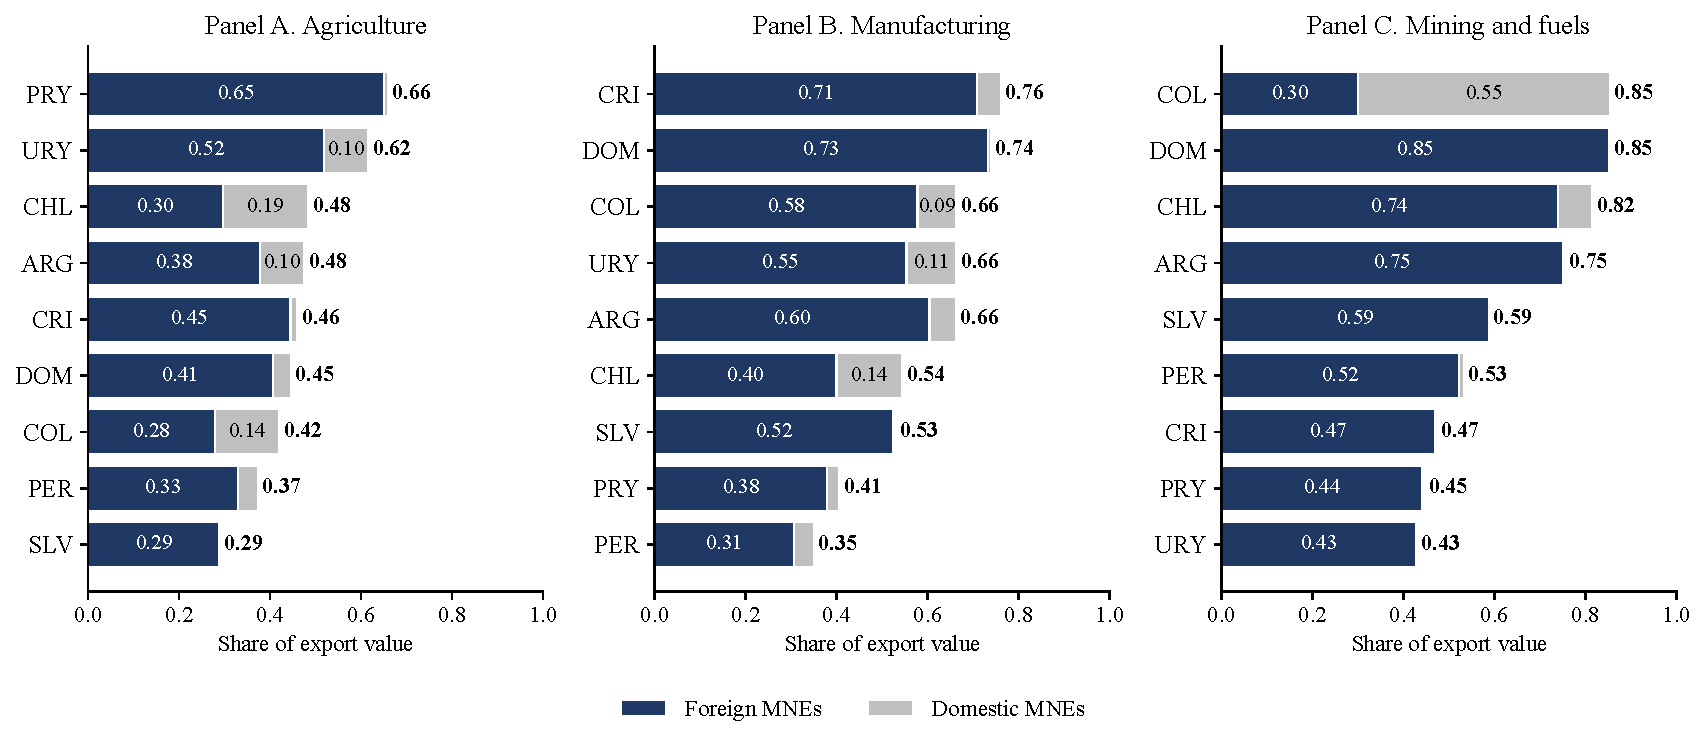
\includegraphics[width=1.0\textwidth,height=0.8\textheight,keepaspectratio]{figures/sectors/fig_wp3_fig1_by_sector_panels.pdf}%
  \caption{Multinational Share of Export Value, by Exporting Country and Sector}%
  \label{fig:a_f1_sectors}%
  \par\vspace{2pt}%
  \parbox{0.92\textwidth}{\footnotesize %
  \textit{Notes:} Shares of each country's export value in the sector. Panel A: agriculture (HS 01--24). Panel B: manufacturing (HS 28--97 excluding 71). Panel C: mining and fuels (HS 25--27 and 71).\\[3pt]%
  \textit{Source:} Authors' calculations based on customs data matched to Orbis and Dun \& Bradstreet.}%
  \end{figure}
% ---- Table: Exports and Multinational Shares, by Sector
\begin{table}[H]\centering\small%
  \caption{Exports and Multinational Shares, by Sector}%
  \label{tab:a_sectors}%
  \adjustbox{max width=\textwidth, max totalheight=0.8\textheight}{\begin{tabular}{@{}l r r r r l@{}}
\toprule
Sector & Total exports (US\$bn/yr) & MNE exports (US\$bn/yr) & Foreign (\%) & Domestic (\%) & Leading parents (share of foreign) \\
\midrule
Agriculture & 78.9 & 37.8 & 38.1 & 9.5 & USA 0.24, CHE 0.11, NLD 0.10 \\
Mining \& fuels & 72.4 & 52.4 & 49.2 & 24.5 & GBR 0.36, USA 0.21, CAN 0.16 \\
Manufacturing & 72.7 & 43.9 & 51.6 & 8.0 & USA 0.25, GBR 0.14, DEU 0.09 \\
Rest & 0.5 & 0.4 & 47.9 & 28.0 & USA 0.39, GBR 0.12, ESP 0.11 \\
\midrule
All & 224.5 & 134.5 & 46.3 & 14.1 & \\
\bottomrule
\end{tabular}
}%
  \par\vspace{3pt}%
  \begin{minipage}{0.95\textwidth}\footnotesize %
  \textit{Notes:} Foreign and domestic: percent of the sector's export value. Rest: HS 98--99 and unclassified codes. Leading parents: the three largest parent countries and their share of the row's foreign-MNE exports. Values are annual averages in US\$ billion.\\[3pt]%
  \textit{Source:} Authors' calculations based on customs data matched to Orbis and Dun \& Bradstreet.%
  \end{minipage}%
  \end{table}

\subsection*{Fact 2}
% ---- Figure: Multinational Share of Export Value, by Product Sophistication and Location of the Parent
\begin{figure}[H]\centering%
  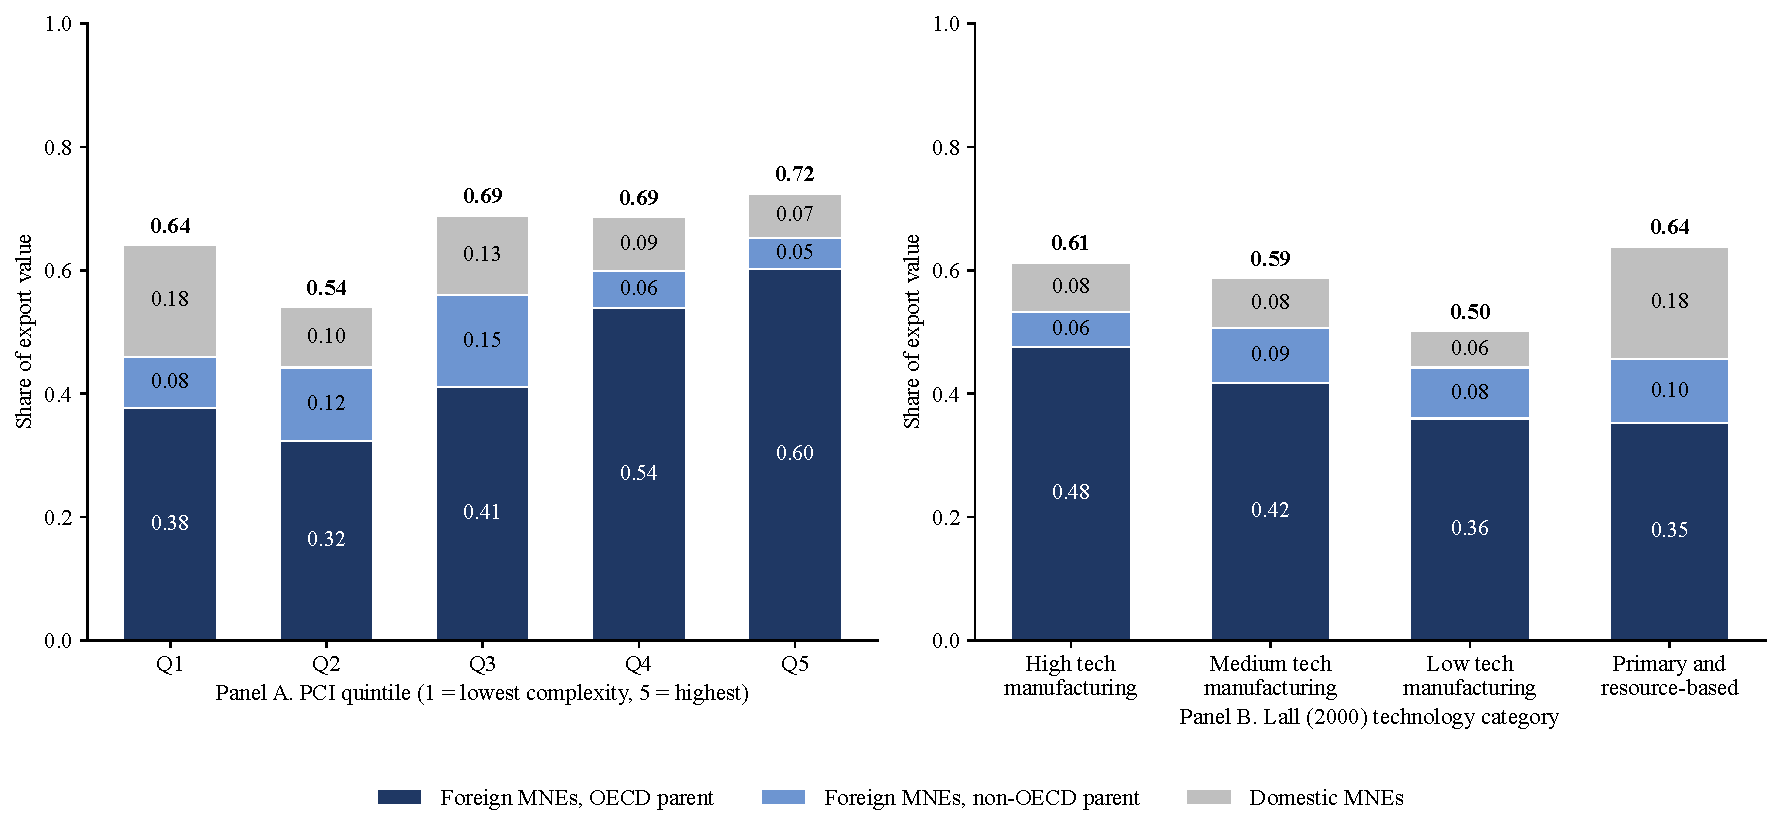
\includegraphics[width=1.0\textwidth,height=0.8\textheight,keepaspectratio]{figures/all/fig_wp1a_pci_lall_by_oecd.pdf}%
  \caption{Multinational Share of Export Value, by Product Sophistication and Location of the Parent}%
  \label{fig:a_f2_oecd}%
  \par\vspace{2pt}%
  \parbox{0.92\textwidth}{\footnotesize %
  \textit{Notes:} Shares of export value, all available years pooled. Foreign MNEs are split by whether the ultimate parent is in an OECD member country. Panel A: Quintiles of the Hausmann--Hidalgo Product Complexity Index across HS6 products (Q1 = least complex). Panel B: Lall (2000) technology classes: primary and resource-based products, and low-, medium- and high-technology manufactures.\\[3pt]%
  \textit{Source:} Authors' calculations based on customs data matched to Orbis and Dun \& Bradstreet.}%
  \end{figure}
% ---- Figure: Manufacturing: Multinational Share of Export Value, by Product Complexity Quintile
\begin{figure}[H]\centering%
  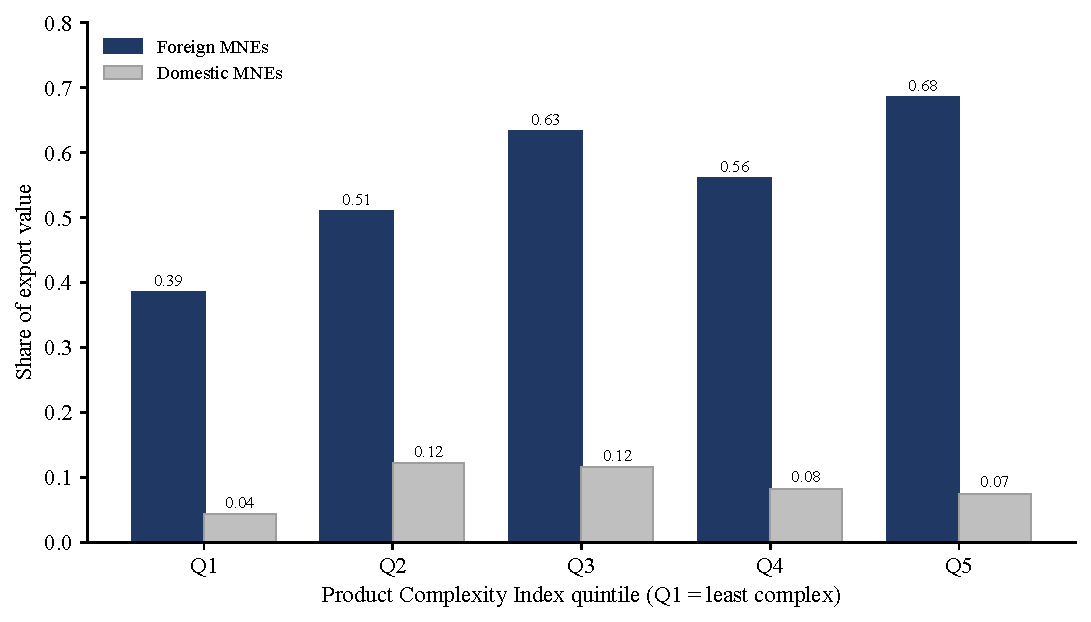
\includegraphics[width=0.78\textwidth,height=0.8\textheight,keepaspectratio]{figures/manufacturing/fig_wp0_fig2_pci.pdf}%
  \caption{Manufacturing: Multinational Share of Export Value, by Product Complexity Quintile}%
  \label{fig:a_f2_manuf}%
  \par\vspace{2pt}%
  \parbox{0.92\textwidth}{\footnotesize %
  \textit{Notes:} Shares of manufacturing export value, all available years pooled. Quintiles computed over manufacturing HS6 products.\\[3pt]%
  \textit{Source:} Authors' calculations based on customs data matched to Orbis and Dun \& Bradstreet.}%
  \end{figure}

\subsection*{Fact 3}
% ---- Table: Destination of Foreign-Multinational Exports, by Parent Country
\begin{table}[H]\centering\small%
  \caption{Destination of Foreign-Multinational Exports, by Parent Country}%
  \label{tab:a_pxd}%
  \adjustbox{max width=\textwidth, max totalheight=0.8\textheight}{\begin{tabular}{lrrrrrrrrrrrr}
\toprule
Parent / Destination & CHN & USA & BRA & JPN & ESP & CHL & KOR & CAN & NLD & ARG & Other destinations & Total \\
\midrule
USA & 10.1 & 22.3 & 7.8 & 3.8 & 4.0 & 2.9 & 2.1 & 0.5 & 3.5 & 4.9 & 38.2 & 100.0 \\
GBR & 36.5 & 5.6 & 3.9 & 7.1 & 3.0 & 3.4 & 6.5 & 3.3 & 3.2 & 0.2 & 27.3 & 100.0 \\
CAN & 12.8 & 6.6 & 4.2 & 5.3 & 3.1 & 0.5 & 1.9 & 19.5 & 0.9 & 0.2 & 45.0 & 100.0 \\
LIE & 24.9 & 3.7 & 3.7 & 18.7 & 3.5 & 2.5 & 5.4 & 0.0 & 1.8 & 0.0 & 35.6 & 100.0 \\
DEU & 1.0 & 14.8 & 31.9 & 1.1 & 1.7 & 3.1 & 0.6 & 1.1 & 1.0 & 0.9 & 42.8 & 100.0 \\
NLD & 9.2 & 3.8 & 26.9 & 0.4 & 1.0 & 3.6 & 1.1 & 0.2 & 2.2 & 3.1 & 48.4 & 100.0 \\
CHE & 6.2 & 5.0 & 6.8 & 0.5 & 2.9 & 3.5 & 0.8 & 0.4 & 2.0 & 0.5 & 71.4 & 100.0 \\
JPN & 2.4 & 8.7 & 45.0 & 8.9 & 0.4 & 1.4 & 0.4 & 0.5 & 0.9 & 1.9 & 29.5 & 100.0 \\
PAN & 35.0 & 9.5 & 1.2 & 1.8 & 1.7 & 1.1 & 6.2 & 0.6 & 2.0 & 0.2 & 40.7 & 100.0 \\
BRA & 12.9 & 14.1 & 18.6 & 1.6 & 0.6 & 3.1 & 0.6 & 0.6 & 2.1 & 2.3 & 43.4 & 100.0 \\
Other parents & 9.5 & 19.5 & 11.7 & 2.2 & 3.7 & 4.0 & 1.6 & 1.6 & 2.1 & 3.7 & 40.3 & 100.0 \\
\bottomrule
\end{tabular}
}%
  \par\vspace{3pt}%
  \begin{minipage}{0.95\textwidth}\footnotesize %
  \textit{Notes:} Percent of each parent country's exports, by destination (rows add to 100). Ten largest parent countries and ten largest destinations by foreign-MNE export value.\\[3pt]%
  \textit{Source:} Authors' calculations based on customs data matched to Orbis and Dun \& Bradstreet.%
  \end{minipage}%
  \end{table}
% ---- Table: Destination of Multinational Exports, by Parent Region
\begin{table}[H]\centering\small%
  \caption{Destination of Multinational Exports, by Parent Region}%
  \label{tab:a_reg}%
  \adjustbox{max width=\textwidth, max totalheight=0.8\textheight}{\begin{tabular}{lrrrrrrrr}
\toprule
Parent region / Destination region & Latin America & North America & Europe & Asia & Africa & Oceania & Rest of World & Total \\
\midrule
Latin America & 40.4 & 15.5 & 14.7 & 27.2 & 1.2 & 0.7 & 0.3 & 100.0 \\
North America & 31.3 & 23.6 & 20.0 & 23.1 & 1.7 & 0.1 & 0.1 & 100.0 \\
Europe & 28.0 & 11.7 & 17.8 & 38.4 & 2.9 & 1.0 & 0.1 & 100.0 \\
Asia & 51.0 & 18.7 & 11.7 & 17.0 & 1.1 & 0.2 & 0.3 & 100.0 \\
Africa & 10.9 & 6.6 & 26.9 & 53.2 & 2.2 & 0.0 & 0.2 & 100.0 \\
Oceania & 20.1 & 5.7 & 8.4 & 65.5 & 0.1 & 0.2 & 0.0 & 100.0 \\
Rest of World & 32.6 & 25.0 & 20.9 & 14.3 & 0.0 & 7.1 & 0.0 & 100.0 \\
Domestic MNEs & 25.9 & 32.9 & 11.1 & 27.0 & 2.3 & 0.5 & 0.3 & 100.0 \\
Local firms & 27.1 & 21.6 & 21.7 & 25.7 & 2.9 & 0.6 & 0.4 & 100.0 \\
\bottomrule
\end{tabular}
}%
  \par\vspace{3pt}%
  \begin{minipage}{0.95\textwidth}\footnotesize %
  \textit{Notes:} Percent of each group's exports, by destination region (rows add to 100). Domestic MNEs and local firms are shown for comparison.\\[3pt]%
  \textit{Source:} Authors' calculations based on customs data matched to Orbis and Dun \& Bradstreet.%
  \end{minipage}%
  \end{table}
% ---- Figure: Destination of Foreign-Multinational Exports: Fifteen Largest Parent Countries and Destinations
\begin{figure}[H]\centering%
  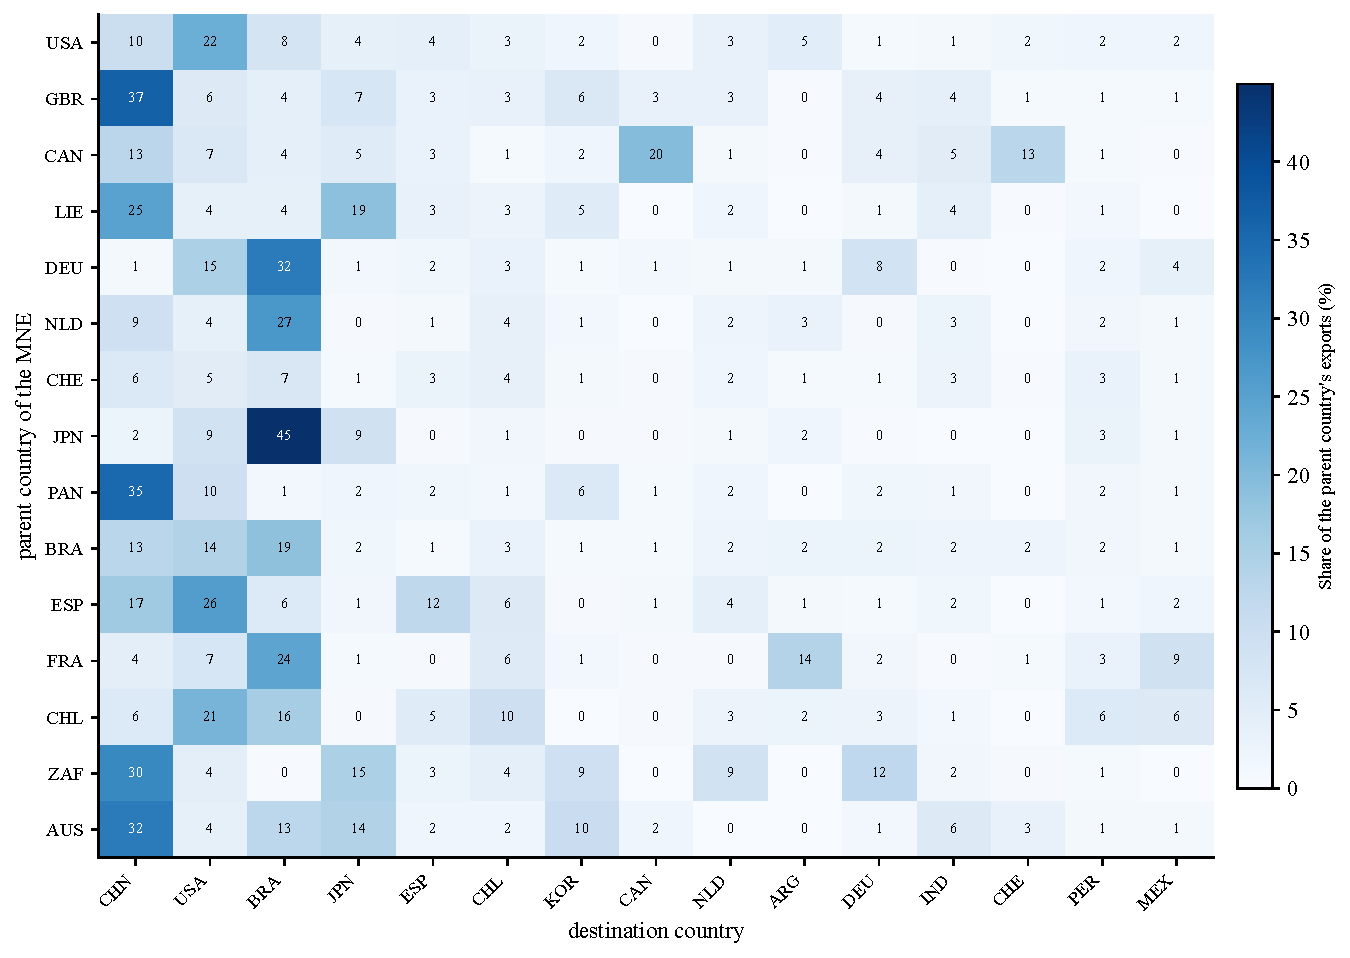
\includegraphics[width=1.0\textwidth,height=0.8\textheight,keepaspectratio]{figures/all/fig_wp1d_heatmap_country_rowpct.pdf}%
  \caption{Destination of Foreign-Multinational Exports: Fifteen Largest Parent Countries and Destinations}%
  \label{fig:a_hm_row}%
  \par\vspace{2pt}%
  \parbox{0.92\textwidth}{\footnotesize %
  \textit{Notes:} Percent of each parent country's exports going to each destination (rows add to 100 including other destinations).\\[3pt]%
  \textit{Source:} Authors' calculations based on customs data matched to Orbis and Dun \& Bradstreet.}%
  \end{figure}
% ---- Figure: Share of Foreign-Multinational Exports Shipped to the Parent Country
\begin{figure}[H]\centering%
  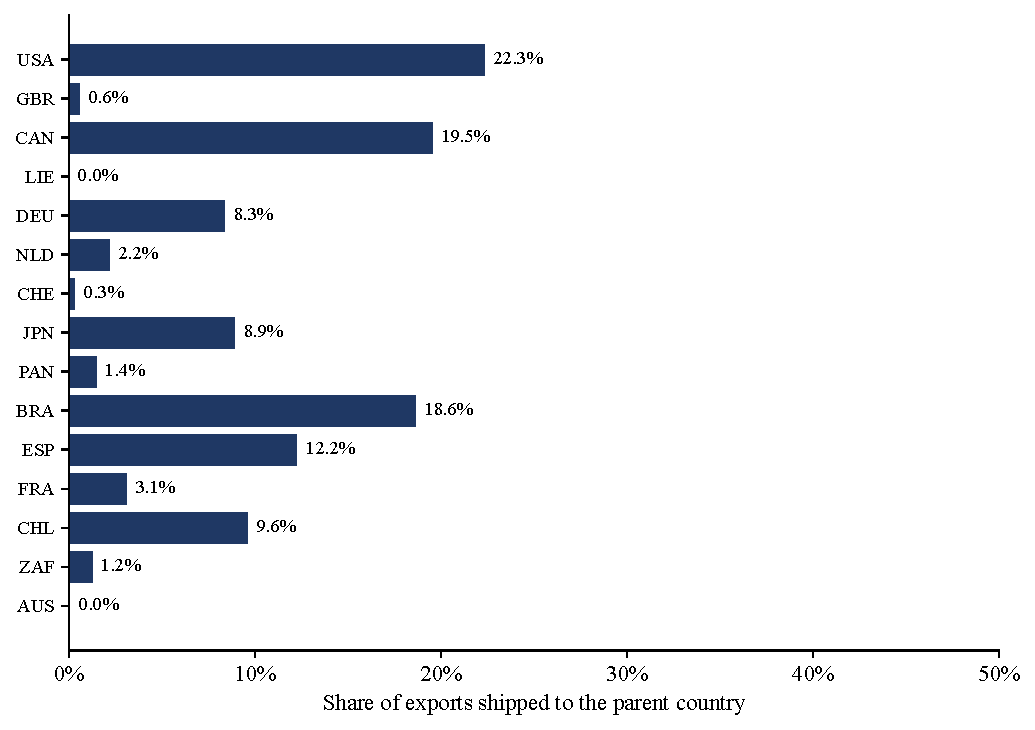
\includegraphics[width=0.85\textwidth,height=0.8\textheight,keepaspectratio]{figures/all/fig_wp1d_home_share_by_parent.pdf}%
  \caption{Share of Foreign-Multinational Exports Shipped to the Parent Country}%
  \label{fig:a_home}%
  \par\vspace{2pt}%
  \parbox{0.92\textwidth}{\footnotesize %
  \textit{Notes:} Percent of each parent country's exports shipped to that same country.\\[3pt]%
  \textit{Source:} Authors' calculations based on customs data matched to Orbis and Dun \& Bradstreet.}%
  \end{figure}
% ---- Figure: Share of Foreign-Multinational Exports Shipped to the Parent Jurisdiction
\begin{figure}[H]\centering%
  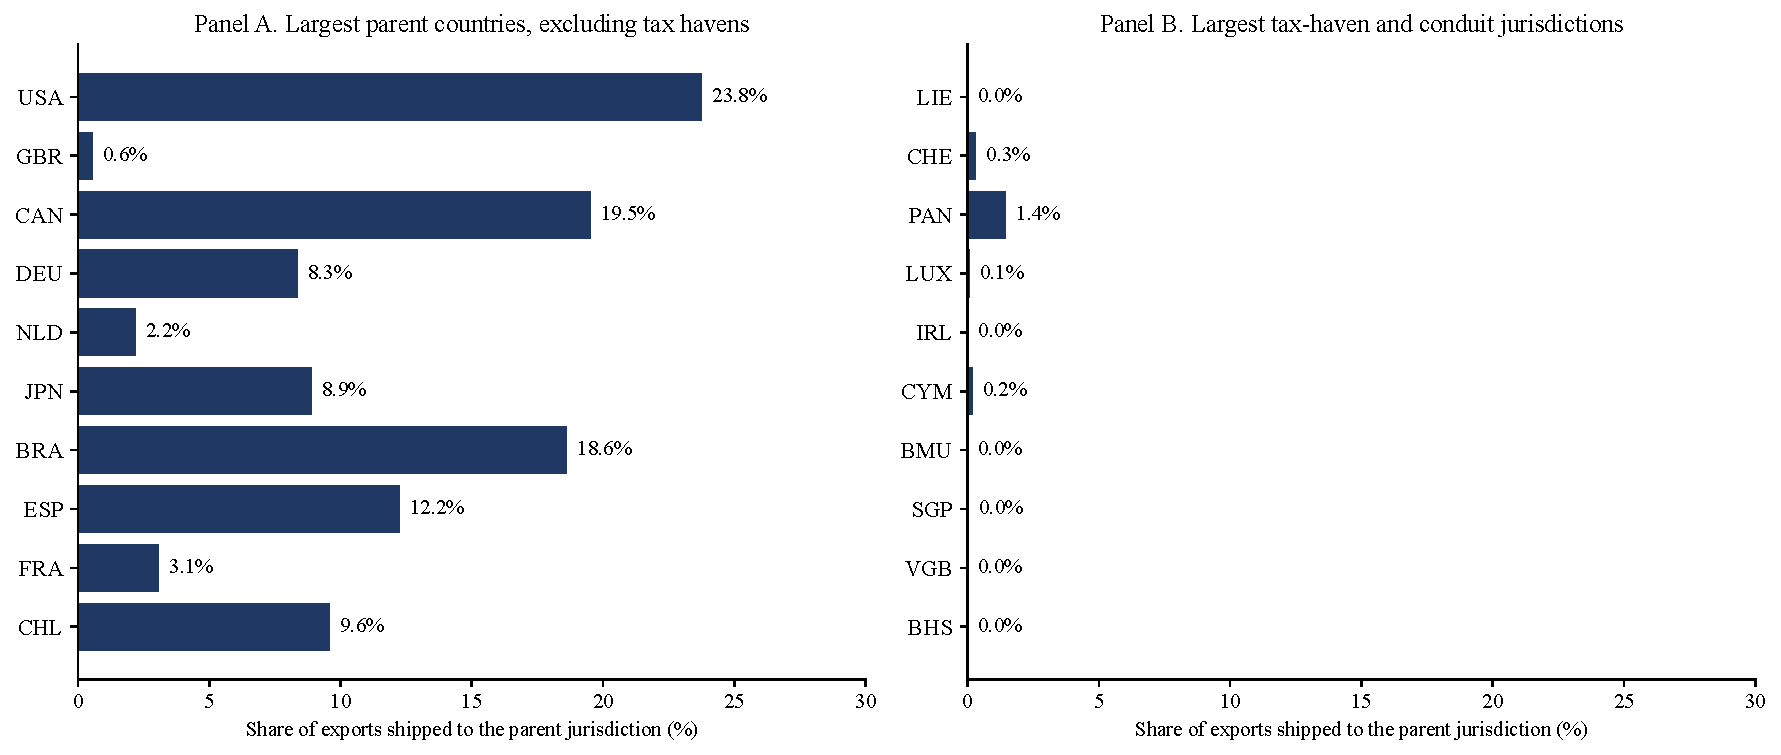
\includegraphics[width=1.0\textwidth,height=0.8\textheight,keepaspectratio]{figures/all/fig_wp1d_home_share_haven_panels.pdf}%
  \caption{Share of Foreign-Multinational Exports Shipped to the Parent Jurisdiction}%
  \label{fig:a_home_havens}%
  \par\vspace{2pt}%
  \parbox{0.92\textwidth}{\footnotesize %
  \textit{Notes:} Percent of each parent jurisdiction's exports shipped to that same jurisdiction. Panel A: largest parent countries, excluding tax havens; dependencies are assigned to their sovereign state. Panel B: largest tax-haven and conduit jurisdictions.\\[3pt]%
  \textit{Source:} Authors' calculations based on customs data matched to Orbis and Dun \& Bradstreet.}%
  \end{figure}
% ---- Figure: Share of Foreign-Multinational Exports Shipped to the Parent Country, by Sector
\begin{figure}[H]\centering%
  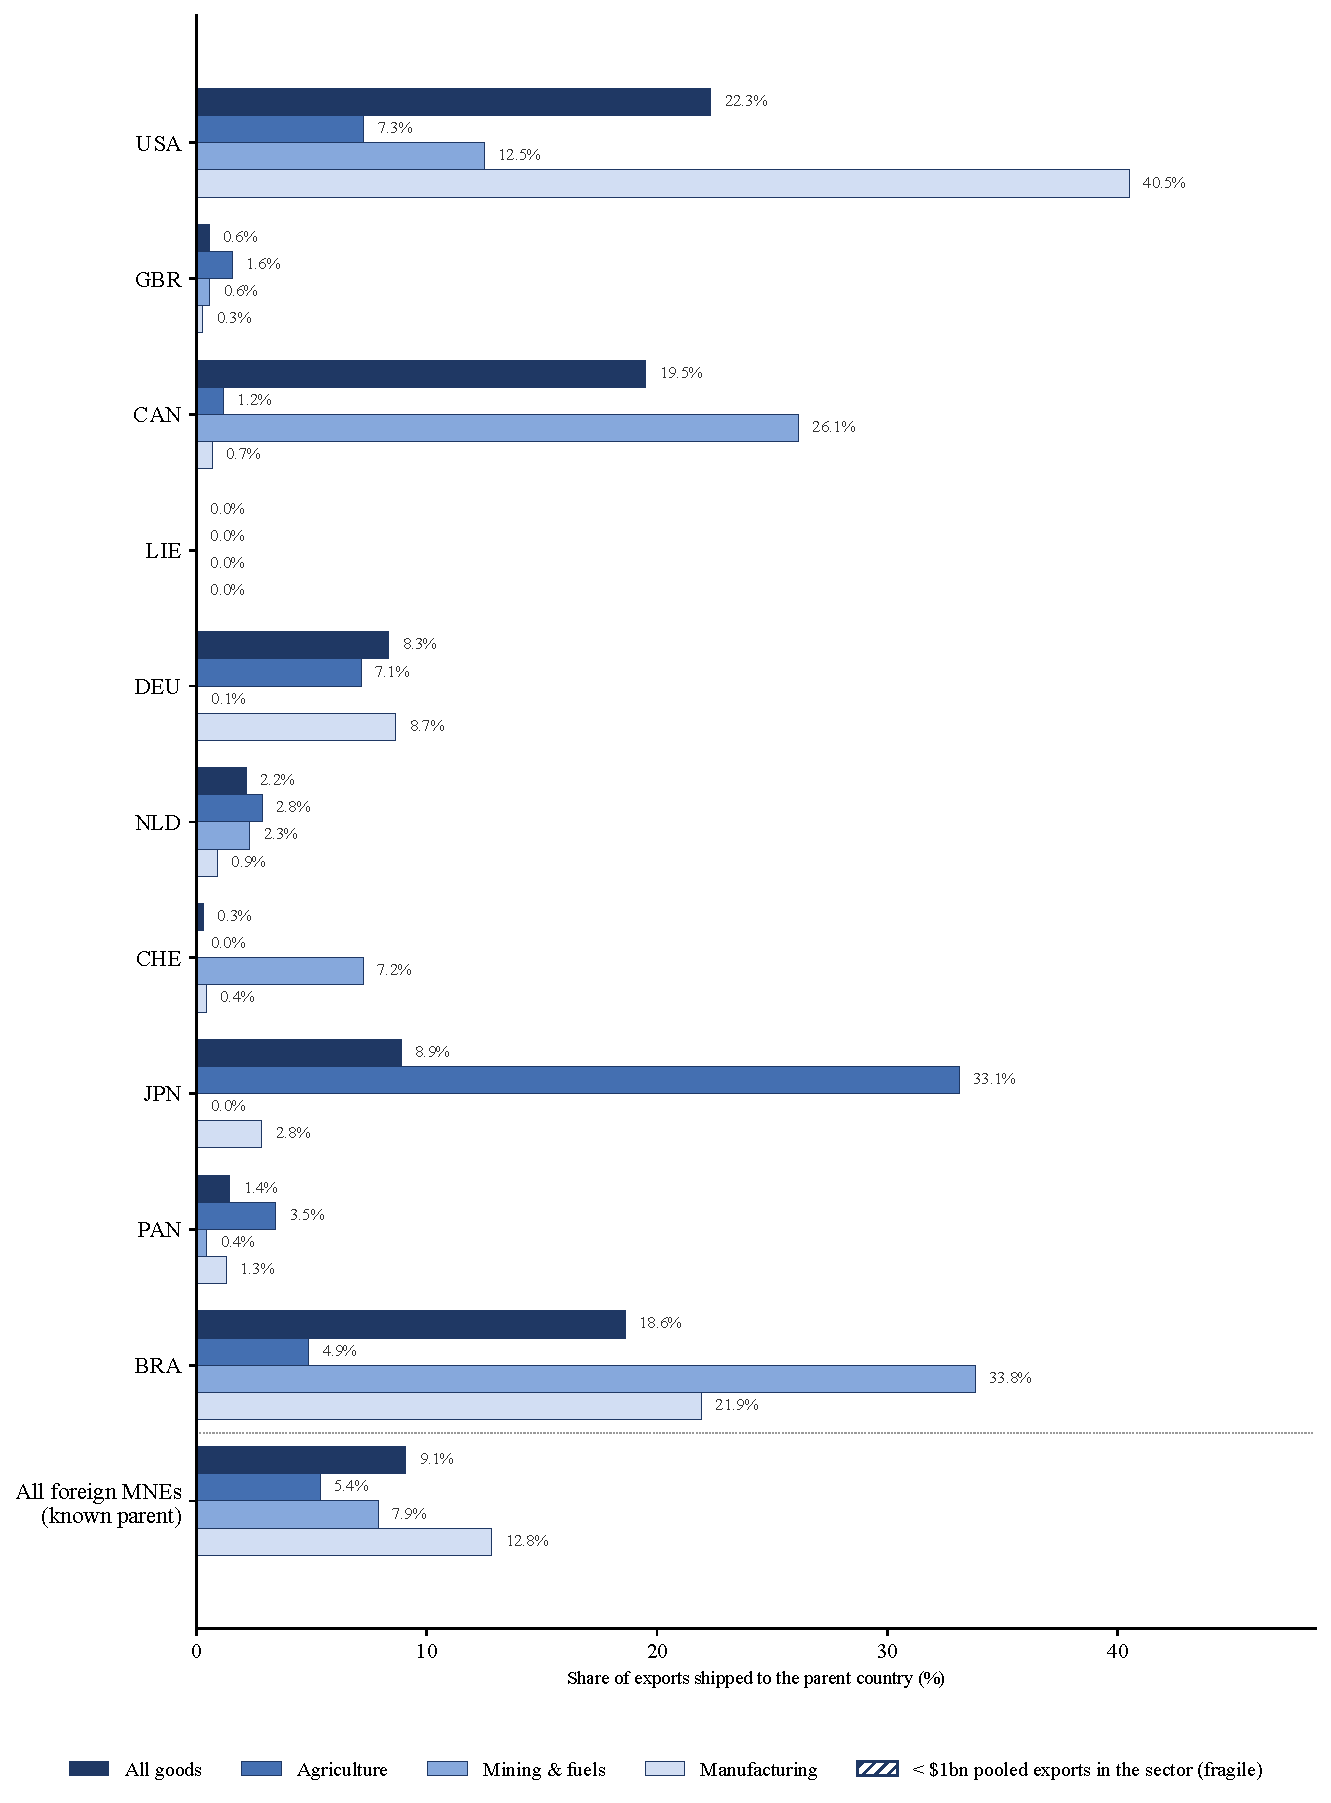
\includegraphics[width=0.95\textwidth,height=0.8\textheight,keepaspectratio]{figures/sectors/fig_wp3_home_share_by_parent_sectors.pdf}%
  \caption{Share of Foreign-Multinational Exports Shipped to the Parent Country, by Sector}%
  \label{fig:a_home_sectors}%
  \par\vspace{2pt}%
  \parbox{0.92\textwidth}{\footnotesize %
  \textit{Notes:} Percent of each parent country's exports shipped to that same country, by sector. Hatched bars: the parent country's exports in the sector are below US\$1 billion over the period.\\[3pt]%
  \textit{Source:} Authors' calculations based on customs data matched to Orbis and Dun \& Bradstreet.}%
  \end{figure}
% ---- Figure: Exports to the United States, by Type of Exporter and Exporting Country
\begin{figure}[H]\centering%
  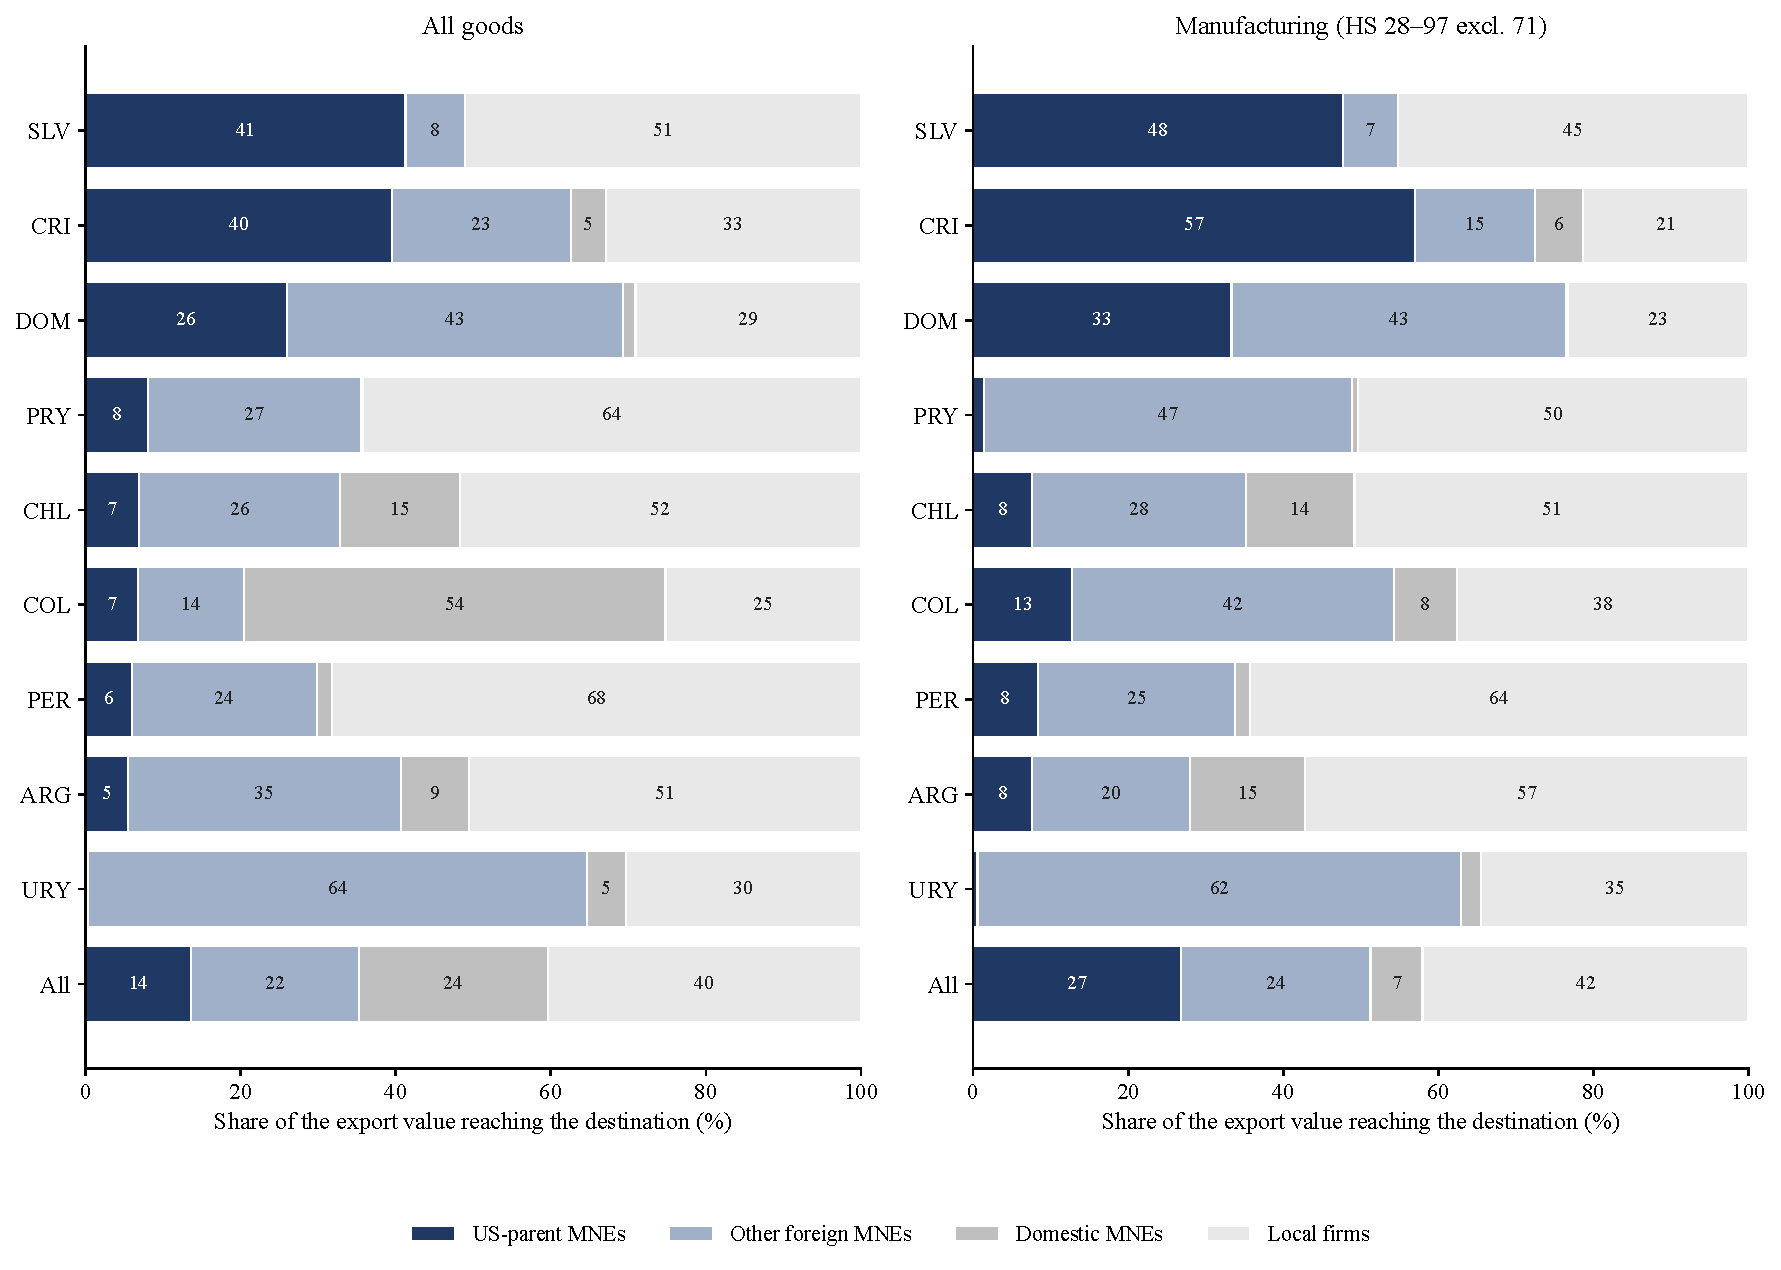
\includegraphics[width=1.0\textwidth,height=0.8\textheight,keepaspectratio]{figures/sectors/fig_wp3_to_usa_carriers_total_manuf.pdf}%
  \caption{Exports to the United States, by Type of Exporter and Exporting Country}%
  \label{fig:a_to_usa}%
  \par\vspace{2pt}%
  \parbox{0.92\textwidth}{\footnotesize %
  \textit{Notes:} Percent of each country's exports to the United States, by type of exporter. Left: all goods. Right: manufacturing.\\[3pt]%
  \textit{Source:} Authors' calculations based on customs data matched to Orbis and Dun \& Bradstreet.}%
  \end{figure}
% ---- Table: Exports to the United States, by Type of Exporter and Sector
\begin{table}[H]\centering\small%
  \caption{Exports to the United States, by Type of Exporter and Sector}%
  \label{tab:a_to_usa_sector}%
  \adjustbox{max width=\textwidth, max totalheight=0.8\textheight}{\begin{tabular}{lrrrrr}
\toprule
Sector & Exports to the USA (US\$bn/yr) & US-parent MNEs (\%) & Other foreign MNEs (\%) & Domestic MNEs (\%) & Local firms (\%) \\
\midrule
\midrule
All goods & 40.0 & 13.6 & 21.6 & 24.4 & 40.4 \\
Agriculture & 10.7 & 4.8 & 28.0 & 9.2 & 58.0 \\
Mining \& fuels & 14.6 & 6.6 & 14.8 & 52.0 & 26.6 \\
Manufacturing & 14.5 & 26.8 & 24.4 & 6.7 & 42.1 \\
Rest & 0.1 & 40.0 & 38.4 & 4.5 & 17.1 \\
\bottomrule
\end{tabular}
}%
  \par\vspace{3pt}%
  \begin{minipage}{0.95\textwidth}\footnotesize %
  \textit{Notes:} Percent of each sector's exports to the United States, by type of exporter. Values are annual averages in US\$ billion.\\[3pt]%
  \textit{Source:} Authors' calculations based on customs data matched to Orbis and Dun \& Bradstreet.%
  \end{minipage}%
  \end{table}
% ---- Table: Main Products Shipped by US-Parent Multinationals to the United States
\begin{table}[H]\centering\footnotesize%
  \caption{Main Products Shipped by US-Parent Multinationals to the United States}%
  \label{tab:a_us_prod}%
  \adjustbox{max width=\textwidth, max totalheight=0.8\textheight}{\begin{tabular}{llrrrrrl}
\toprule
HS6 & Description & \multicolumn{1}{p{1.7cm}}{\raggedright US-parent exports to the USA (US\$bn/yr)} & \multicolumn{1}{p{1.7cm}}{\raggedright \% of all US-parent exports to the USA} & \multicolumn{1}{p{2.0cm}}{\raggedright \% of US-parent exports of the line going to the USA} & \multicolumn{1}{p{1.9cm}}{\raggedright All LAC exports of the line to the USA (US\$bn/yr)} & \multicolumn{1}{p{2.2cm}}{\raggedright US-parent share of LAC exports of the line to the USA (\%)} & \multicolumn{1}{p{2.6cm}}{\raggedright Main origins of the US-parent shipments (\% of the line)} \\
\midrule
610910 & T-shirts, singlets \& other vests, knitted/cro... & 0.49 & 11.1 & 84 & 1.01 & 53 & SLV 85\%, DOM 10\%, PER 5\% \\
901839 & Catheters, cannulae \& the like & 0.52 & 9.6 & 73 & 0.63 & 89 & CRI 92\%, DOM 8\%, COL 0\% \\
270900 & Petroleum oils \& oils obt. from bituminous mi... & 0.41 & 9.1 & 24 & 7.84 & 5 & COL 100\%, ARG 0\% \\
901890 & Instruments \& appliances used in medical/surg... & 0.39 & 6.8 & 69 & 0.94 & 47 & CRI 71\%, DOM 29\%, COL 0\% \\
270112 & Bituminous coal, whether/not pulverised but n... & 0.19 & 4.3 & 9 & 0.39 & 48 & COL 100\% \\
854231 & Electronic integrated circuits, processors \& ... & 0.21 & 3.9 & 28 & 0.22 & 95 & CRI 100\%, COL 0\%, ARG 0\% \\
401110 & New pneumatic tyres, of rubber, of a kind use... & 0.13 & 3.4 & 93 & 0.24 & 63 & CHL 100\%, DOM 0\%, COL 0\% \\
261390 & Molybdenum ores \& concentrates, other than ro... & 0.15 & 2.8 & 99 & 0.18 & 79 & PER 100\% \\
611595 & Other n.e.s. in 61.15, knitted/crocheted, of ... & 0.10 & 2.4 & 100 & 0.11 & 97 & SLV 100\%, DOM 0\% \\
610711 & Men's/boys' underpants \& briefs, knitted/croc... & 0.09 & 2.2 & 87 & 0.10 & 87 & SLV 100\%, DOM 0\%, CRI 0\% \\
621210 & Brassieres \& parts thereof , whether/not knit... & 0.09 & 1.8 & 98 & 0.12 & 78 & SLV 74\%, DOM 26\%, CRI 0\% \\
080430 & Pineapples, fresh/dried & 0.08 & 1.6 & 66 & 0.42 & 20 & CRI 100\% \\
240210 & Cigars, cheroots \& cigarillos containing toba... & 0.09 & 1.3 & 100 & 0.57 & 16 & DOM 100\% \\
740311 & Cathodes \& sections of cathodes, of refined c... & 0.06 & 1.2 & 24 & 1.56 & 3 & PER 64\%, CHL 36\% \\
640510 & Footwear with uppers of leather/composition l... & 0.08 & 1.2 & 70 & 0.11 & 71 & DOM 100\% \\
\midrule
All lines & & 5.0 & 100.0 & 22 & 40.0 & 14 & \\
\bottomrule
\end{tabular}
}%
  \par\vspace{3pt}%
  \begin{minipage}{0.95\textwidth}\footnotesize %
  \textit{Notes:} Fifteen HS6 products with the largest exports by US-parent MNEs to the United States. Values are annual averages in US\$ billion.\\[3pt]%
  \textit{Source:} Authors' calculations based on customs data matched to Orbis and Dun \& Bradstreet.%
  \end{minipage}%
  \end{table}

\subsection*{Fact 4}
% ---- Table: Foreign-Multinational Exports and Number of Parents, by Size of the Group's Global Network
\begin{table}[H]\centering\small%
  \caption{Foreign-Multinational Exports and Number of Parents, by Size of the Group's Global Network}%
  \label{tab:a_f5_tab}%
  \adjustbox{max width=\textwidth, max totalheight=0.8\textheight}{\begin{tabular}{lrrr}
\toprule
Affiliates worldwide & Parents & Share of parents (\%) & Share of foreign-MNE export value (\%) \\
\midrule
1 & 5,982 & 48.4 & 5.4 \\
2--10 & 3,397 & 27.5 & 12.4 \\
11--100 & 1,893 & 15.3 & 26.2 \\
$>$100 & 1,099 & 8.9 & 56.0 \\
\midrule
All parents & 12,371 & 100 & 100 \\
\bottomrule
\end{tabular}
}%
  \par\vspace{3pt}%
  \begin{minipage}{0.95\textwidth}\footnotesize %
  \textit{Notes:} Number and share of parents, and share of foreign-MNE export value, by the number of affiliates the group has worldwide. Parents with a network record in Orbis or Dun \& Bradstreet: 98 percent of parents and 97 percent of foreign-MNE export value.\\[3pt]%
  \textit{Source:} Authors' calculations based on customs data matched to Orbis and Dun \& Bradstreet.%
  \end{minipage}%
  \end{table}

\subsection*{Fact 5}
% ---- Table: Multinational Presence and Exports: Extensive Margin, by Type of Multinational
\begin{table}[H]\centering\small%
  \caption{Multinational Presence and Exports: Extensive Margin, by Type of Multinational}%
  \label{tab:a_ext}%
  \adjustbox{max width=\textwidth, max totalheight=0.8\textheight}{\begin{tabular}{lcccccc} \hline
 & \multicolumn{2}{c}{All MNEs} & \multicolumn{2}{c}{Foreign / domestic} & \multicolumn{2}{c}{Foreign by destination, domestic} \\
 & (1) & (2) & (3) & (4) & (5) & (6) \\ \hline
\multicolumn{7}{l}{\textit{Panel A. Dependent variable: $\ln$ exports, all firms}} \\
Any MNE present & 1.4591*** & 0.6818*** &  &  &  &  \\
 & (0.0388) & (0.0165) &  &  &  &  \\
Any foreign MNE &  &  & 1.4990*** & 0.6986*** &  &  \\
 &  &  & (0.0339) & (0.0158) &  &  \\
Any foreign MNE, parent-country destination &  &  &  &  & 1.3873*** & 0.5909*** \\
 &  &  &  &  & (0.0951) & (0.0431) \\
Any foreign MNE, other destination &  &  &  &  & 1.5093*** & 0.6976*** \\
 &  &  &  &  & (0.0319) & (0.0146) \\
Any domestic MNE &  &  & 1.4670*** & 0.4917*** & 1.4334*** & 0.4909*** \\
 &  &  & (0.0416) & (0.0165) & (0.0388) & (0.0166) \\
\midrule
\multicolumn{7}{l}{\textit{Panel B. Dependent variable: $\ln$ exports, non-MNE firms}} \\
Any MNE present & 1.3996*** & 0.1311*** &  &  &  &  \\
 & (0.0367) & (0.0102) &  &  &  &  \\
Any foreign MNE &  &  & 1.2983*** & 0.1356*** &  &  \\
 &  &  & (0.0346) & (0.0106) &  &  \\
Any foreign MNE, parent-country destination &  &  &  &  & 1.0183*** & 0.1265*** \\
 &  &  &  &  & (0.0900) & (0.0194) \\
Any foreign MNE, other destination &  &  &  &  & 1.2782*** & 0.1386*** \\
 &  &  &  &  & (0.0326) & (0.0107) \\
Any domestic MNE &  &  & 1.1316*** & 0.1370*** & 1.0959*** & 0.1367*** \\
 &  &  & (0.0428) & (0.0138) & (0.0403) & (0.0138) \\
\hline
Product FE & $\checkmark$ &  & $\checkmark$ &  & $\checkmark$ &  \\
Origin $\times$ year FE & $\checkmark$ &  & $\checkmark$ &  & $\checkmark$ &  \\
Destination $\times$ year FE & $\checkmark$ &  & $\checkmark$ &  & $\checkmark$ &  \\
Origin $\times$ dest.\ $\times$ product FE &  & $\checkmark$ &  & $\checkmark$ &  & $\checkmark$ \\
Origin $\times$ dest.\ $\times$ year FE &  & $\checkmark$ &  & $\checkmark$ &  & $\checkmark$ \\
Observations (Panel A) & 1,829,626 & 1,633,319 & 1,829,626 & 1,633,319 & 1,829,626 & 1,633,319 \\
Observations (Panel B) & 1,297,111 & 1,137,550 & 1,297,111 & 1,137,550 & 1,297,111 & 1,137,550 \\
\hline
\end{tabular}
}%
  \par\vspace{3pt}%
  \begin{minipage}{0.95\textwidth}\footnotesize %
  \textit{Notes:} Observations are origin--destination--HS6--year cells. Dependent variable: $\ln$ exports of the cell (Panel A) and of the non-MNE firms in the cell (Panel B). Regressors: indicators for at least one MNE of each type. Columns (5)--(6) split foreign MNEs by whether the destination is the parent's country. Standard errors clustered by origin--destination pair in parentheses. *** $p<0.01$, ** $p<0.05$, * $p<0.1$.\\[3pt]%
  \textit{Source:} Authors' calculations based on customs data matched to Orbis and Dun \& Bradstreet.%
  \end{minipage}%
  \end{table}
% ---- Table: Multinational Exports by Exporting Country and Destination Type
\begin{table}[H]\centering\small%
  \caption{Multinational Exports by Exporting Country and Destination Type}%
  \label{tab:a_pres}%
  \adjustbox{max width=\textwidth, max totalheight=0.8\textheight}{\begin{tabular}{lrrrrr}
\toprule
Origin & MNE value (US\$bn/yr) & of which domestic (\%) & Foreign-MNE value (US\$bn/yr) & \multicolumn{2}{c}{\% of foreign-MNE value, by destination} \\
 & & & & parent country & other (of which: group affiliate there) \\
\midrule
ARG & 37.5 & 13.3 & 32.5 & 6.5 & 93.5 (41.8) \\
CHL & 21.0 & 22.1 & 16.4 & 4.3 & 95.7 (56.7) \\
COL & 32.8 & 52.5 & 15.5 & 6.5 & 93.5 (34.2) \\
CRI & 6.6 & 5.7 & 6.3 & 25.5 & 74.5 (33.8) \\
DOM & 6.0 & 1.8 & 5.9 & 29.0 & 71.0 (21.6) \\
PER & 19.3 & 5.0 & 18.3 & 3.9 & 96.1 (28.8) \\
PRY & 4.5 & 1.8 & 4.4 & 2.1 & 97.9 (65.5) \\
SLV & 2.4 & 0.6 & 2.4 & 40.7 & 59.3 (28.1) \\
URY & 4.4 & 15.9 & 3.7 & 5.2 & 94.8 (37.7) \\
\midrule
All & 134.5 & 23.4 & 105.4 & 8.4 & 91.6 (40.5) \\
\bottomrule
\end{tabular}
}%
  \par\vspace{3pt}%
  \begin{minipage}{0.95\textwidth}\footnotesize %
  \textit{Notes:} MNE and foreign-MNE export value by country, and the split of foreign-MNE value by destination. Parent country: exports to the country of the ultimate parent. Other: all remaining destinations; in parentheses, destinations where the group has another affiliate. Values are annual averages in US\$ billion.\\[3pt]%
  \textit{Source:} Authors' calculations based on customs data matched to Orbis and Dun \& Bradstreet.%
  \end{minipage}%
  \end{table}
% ---- Table: Multinational Presence and Exports by Sector: Intensive Margin
\begin{table}[H]\centering\small%
  \caption{Multinational Presence and Exports by Sector: Intensive Margin}%
  \label{tab:a_f5sum}%
  \adjustbox{max width=\textwidth, max totalheight=0.8\textheight}{\begin{tabular}{lcccc} \hline
Sample & All goods & Agriculture & Mining \& fuels & Manufacturing \\ \hline
\multicolumn{5}{l}{\textit{Panel A. Dependent variable: $\ln$ exports, all firms}} \\
\multicolumn{5}{l}{\footnotesize Fixed effects: origin $\times$ year, destination $\times$ year, product} \\
\quad $\ln$(\# foreign MNEs) & 1.2129*** & 1.2954*** & 1.1301*** & 1.1644*** \\
 & (0.0285) & (0.0275) & (0.1799) & (0.0358) \\
\quad $\ln$(\# domestic MNEs) & 0.4382*** & 0.5233*** & 0.3172 & 0.3833*** \\
 & (0.0259) & (0.0266) & (0.2062) & (0.0319) \\
\quad Observations & 113,422 & 25,437 & 1,417 & 85,453 \\
\multicolumn{5}{l}{\footnotesize Fixed effects: origin $\times$ destination $\times$ product, origin $\times$ destination $\times$ year} \\
\quad $\ln$(\# foreign MNEs) & 0.4506*** & 0.4625*** & 0.2479 & 0.4435*** \\
 & (0.0124) & (0.0188) & (0.1778) & (0.0148) \\
\quad $\ln$(\# domestic MNEs) & 0.2214*** & 0.2831*** & 0.3216* & 0.1904*** \\
 & (0.0151) & (0.0234) & (0.1639) & (0.0175) \\
\quad Observations & 98,223 & 22,002 & 1,027 & 73,318 \\
\midrule
\multicolumn{5}{l}{\textit{Panel B. Dependent variable: $\ln$ exports, non-MNE firms}} \\
\multicolumn{5}{l}{\footnotesize Fixed effects: origin $\times$ year, destination $\times$ year, product} \\
\quad $\ln$(\# foreign MNEs) & 1.1331*** & 1.2191*** & 0.9420*** & 1.0546*** \\
 & (0.0375) & (0.0363) & (0.2641) & (0.0493) \\
\quad $\ln$(\# domestic MNEs) & 0.4707*** & 0.5676*** & -0.6594 & 0.4194*** \\
 & (0.0341) & (0.0339) & (0.4830) & (0.0419) \\
\quad Observations & 93,010 & 22,503 & 995 & 68,534 \\
\multicolumn{5}{l}{\footnotesize Fixed effects: origin $\times$ destination $\times$ product, origin $\times$ destination $\times$ year} \\
\quad $\ln$(\# foreign MNEs) & 0.2413*** & 0.3602*** & -0.1512 & 0.1865*** \\
 & (0.0217) & (0.0292) & (0.3320) & (0.0250) \\
\quad $\ln$(\# domestic MNEs) & 0.1250*** & 0.2461*** & -0.7273 & 0.0742*** \\
 & (0.0218) & (0.0341) & (0.6536) & (0.0238) \\
\quad Observations & 81,563 & 19,535 & 726 & 59,772 \\
\hline
\end{tabular}
}%
  \par\vspace{3pt}%
  \begin{minipage}{0.95\textwidth}\footnotesize %
  \textit{Notes:} Observations are origin--destination--HS6--year cells. Dependent variable: $\ln$ exports of the cell (Panel A) and of the non-MNE firms in the cell (Panel B). Specification of columns (3)--(4) of Table~\ref{tab:p_f5counts}, estimated by sector. Blank: too few observations. Standard errors clustered by origin--destination pair in parentheses. *** $p<0.01$, ** $p<0.05$, * $p<0.1$.\\[3pt]%
  \textit{Source:} Authors' calculations based on customs data matched to Orbis and Dun \& Bradstreet.%
  \end{minipage}%
  \end{table}
% ---- Table: Multinational Presence and Exports by Sector: Extensive Margin
\begin{table}[H]\centering\small%
  \caption{Multinational Presence and Exports by Sector: Extensive Margin}%
  \label{tab:a_f5extsum}%
  \adjustbox{max width=\textwidth, max totalheight=0.8\textheight}{\begin{tabular}{lcccc} \hline
Sample & All goods & Agriculture & Mining \& fuels & Manufacturing \\ \hline
\multicolumn{5}{l}{\textit{Panel A. Dependent variable: $\ln$ exports, all firms}} \\
\multicolumn{5}{l}{\footnotesize Fixed effects: origin $\times$ year, destination $\times$ year, product} \\
\quad At least one foreign MNE exports the product to the destination (0/1) & 1.4990*** & 1.7972*** & 1.4255*** & 1.4231*** \\
 & (0.0339) & (0.0558) & (0.0892) & (0.0344) \\
\quad At least one domestic MNE exports the product to the destination (0/1) & 1.4670*** & 1.6133*** & 1.7356*** & 1.3878*** \\
 & (0.0416) & (0.0577) & (0.1413) & (0.0466) \\
\quad Observations & 1,829,626 & 295,788 & 32,912 & 1,496,381 \\
\multicolumn{5}{l}{\footnotesize Fixed effects: origin $\times$ destination $\times$ product, origin $\times$ destination $\times$ year} \\
\quad At least one foreign MNE exports the product to the destination (0/1) & 0.6986*** & 0.6929*** & 0.7311*** & 0.7021*** \\
 & (0.0158) & (0.0213) & (0.0560) & (0.0178) \\
\quad At least one domestic MNE exports the product to the destination (0/1) & 0.4917*** & 0.5683*** & 0.5718*** & 0.4684*** \\
 & (0.0165) & (0.0237) & (0.1044) & (0.0186) \\
\quad Observations & 1,633,319 & 268,332 & 27,664 & 1,329,815 \\
\midrule
\multicolumn{5}{l}{\textit{Panel B. Dependent variable: $\ln$ exports, non-MNE firms}} \\
\multicolumn{5}{l}{\footnotesize Fixed effects: origin $\times$ year, destination $\times$ year, product} \\
\quad At least one foreign MNE exports the product to the destination (0/1) & 1.2983*** & 1.7649*** & 1.5696*** & 1.1402*** \\
 & (0.0346) & (0.0546) & (0.1099) & (0.0344) \\
\quad At least one domestic MNE exports the product to the destination (0/1) & 1.1316*** & 1.3082*** & 1.1333*** & 1.0491*** \\
 & (0.0428) & (0.0539) & (0.1497) & (0.0490) \\
\quad Observations & 1,297,111 & 232,617 & 22,836 & 1,038,206 \\
\multicolumn{5}{l}{\footnotesize Fixed effects: origin $\times$ destination $\times$ product, origin $\times$ destination $\times$ year} \\
\quad At least one foreign MNE exports the product to the destination (0/1) & 0.1356*** & 0.2854*** & 0.1991*** & 0.0997*** \\
 & (0.0106) & (0.0179) & (0.0547) & (0.0114) \\
\quad At least one domestic MNE exports the product to the destination (0/1) & 0.1370*** & 0.2610*** & 0.2125** & 0.0984*** \\
 & (0.0138) & (0.0201) & (0.0899) & (0.0167) \\
\quad Observations & 1,137,550 & 208,479 & 18,666 & 904,114 \\
\hline
\end{tabular}
}%
  \par\vspace{3pt}%
  \begin{minipage}{0.95\textwidth}\footnotesize %
  \textit{Notes:} Observations are origin--destination--HS6--year cells. Dependent variable: $\ln$ exports of the cell (Panel A) and of the non-MNE firms in the cell (Panel B). Specification of columns (3)--(4) of Table~\ref{tab:a_ext}, estimated by sector. Standard errors clustered by origin--destination pair in parentheses. *** $p<0.01$, ** $p<0.05$, * $p<0.1$.\\[3pt]%
  \textit{Source:} Authors' calculations based on customs data matched to Orbis and Dun \& Bradstreet.%
  \end{minipage}%
  \end{table}

\subsection*{Fact 6}
% ---- Table: Distance and Firm Exports, by Sector
\begin{table}[H]\centering\small%
  \caption{Distance and Firm Exports, by Sector}%
  \label{tab:a_f6sum}%
  \adjustbox{max width=\textwidth, max totalheight=0.8\textheight}{\begin{tabular}{lcccc} \hline
Dep.\ var.: $\ln$ firm exports & All goods & Agriculture & Mining \& fuels & Manufacturing \\ \hline
\multicolumn{5}{l}{\footnotesize Origin, destination, year and product FE} \\
\quad $\ln$ distance & -0.1645*** & -0.2135*** & -0.0926 & -0.1510*** \\
 & (0.0454) & (0.0748) & (0.0819) & (0.0454) \\
\quad $\ln$ distance $\times$ foreign MNE & 0.0487*** & 0.0366*** & 0.0566*** & 0.0515*** \\
 & (0.0041) & (0.0034) & (0.0086) & (0.0048) \\
\quad $\ln$ distance $\times$ domestic MNE & 0.0318*** & 0.0187*** & 0.0706*** & 0.0388*** \\
 & (0.0042) & (0.0046) & (0.0180) & (0.0052) \\
\quad Observations & 5,081,547 & 1,045,009 & 79,938 & 3,917,960 \\
\midrule
\multicolumn{5}{l}{\footnotesize Origin $\times$ year, destination $\times$ year and product FE} \\
\quad $\ln$ distance & -0.1853*** & -0.2285*** & -0.1001 & -0.1742*** \\
 & (0.0460) & (0.0711) & (0.0828) & (0.0459) \\
\quad $\ln$ distance $\times$ foreign MNE & 0.0483*** & 0.0358*** & 0.0557*** & 0.0512*** \\
 & (0.0040) & (0.0034) & (0.0087) & (0.0048) \\
\quad $\ln$ distance $\times$ domestic MNE & 0.0318*** & 0.0182*** & 0.0673*** & 0.0390*** \\
 & (0.0042) & (0.0046) & (0.0183) & (0.0052) \\
\quad Observations & 5,081,360 & 1,044,787 & 79,612 & 3,917,765 \\
\hline
\end{tabular}
}%
  \par\vspace{3pt}%
  \begin{minipage}{0.95\textwidth}\footnotesize %
  \textit{Notes:} Observations are firm--destination--HS6--year cells. Dependent variable: $\ln$ exports. Specification of columns (1)--(2) of Table~\ref{tab:p_dist}, estimated by sector. Standard errors clustered by origin--destination pair in parentheses. *** $p<0.01$, ** $p<0.05$, * $p<0.1$.\\[3pt]%
  \textit{Source:} Authors' calculations based on customs data matched to Orbis and Dun \& Bradstreet.%
  \end{minipage}%
  \end{table}

\subsection*{Products}
% ---- Figure: Distribution of Export Value by Product-Level Foreign-Multinational Share
\begin{figure}[H]\centering%
  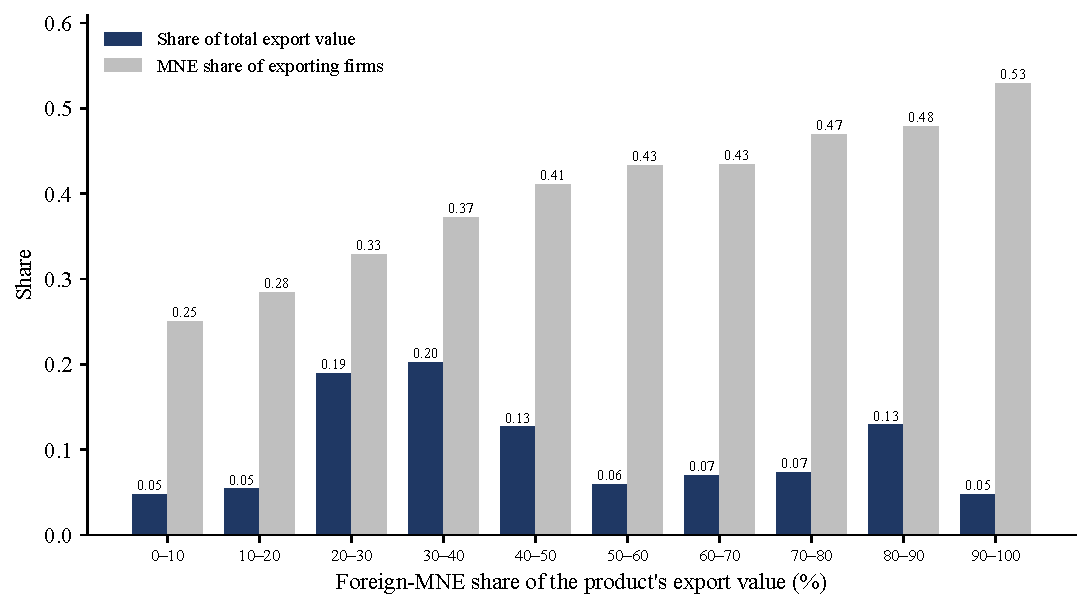
\includegraphics[width=0.85\textwidth,height=0.8\textheight,keepaspectratio]{figures/all/fig_wp1f_foreign_share_distribution.pdf}%
  \caption{Distribution of Export Value by Product-Level Foreign-Multinational Share}%
  \label{fig:a_dist}%
  \par\vspace{2pt}%
  \parbox{0.92\textwidth}{\footnotesize %
  \textit{Notes:} Share of total export value and MNE share of exporting firms, by the foreign-MNE share of each HS6 product's export value.\\[3pt]%
  \textit{Source:} Authors' calculations based on customs data matched to Orbis and Dun \& Bradstreet.}%
  \end{figure}
% ---- Table: Distribution of Export Value by Product-Level Foreign-Multinational Share
\begin{table}[H]\centering\small%
  \caption{Distribution of Export Value by Product-Level Foreign-Multinational Share}%
  \label{tab:a_dist_tab}%
  \adjustbox{max width=\textwidth, max totalheight=0.8\textheight}{\begin{tabular}{lrrr}
\toprule
Foreign share bin (\%) & Share of value & MNE share of exporting firms & HS6 products \\
\midrule
0--10 & 0.048 & 0.250 & 1,426 \\
10--20 & 0.054 & 0.285 & 731 \\
20--30 & 0.189 & 0.329 & 652 \\
30--40 & 0.202 & 0.372 & 591 \\
40--50 & 0.127 & 0.411 & 519 \\
50--60 & 0.059 & 0.433 & 442 \\
60--70 & 0.070 & 0.435 & 386 \\
70--80 & 0.074 & 0.470 & 311 \\
80--90 & 0.129 & 0.479 & 311 \\
90--100 & 0.048 & 0.530 & 560 \\
\bottomrule
\end{tabular}
}%
  \par\vspace{3pt}%
  \begin{minipage}{0.95\textwidth}\footnotesize %
  \textit{Notes:} Share of total export value and MNE share of exporting firms, by the foreign-MNE share of each HS6 product's export value. MNE share of exporting firms: MNE firm--destination--product--year observations over all observations in the bin.\\[3pt]%
  \textit{Source:} Authors' calculations based on customs data matched to Orbis and Dun \& Bradstreet.%
  \end{minipage}%
  \end{table}
% ---- Table: Agriculture: Exports and Multinational Shares, by SITC Division
\begin{table}[H]\centering\footnotesize%
  \caption{Agriculture: Exports and Multinational Shares, by SITC Division}%
  \label{tab:a_agro_sitc}%
  \adjustbox{max width=\textwidth, max totalheight=0.8\textheight}{\begin{tabular}{@{}l r r r r l@{}}
\toprule
SITC Rev.\,3 division & Total exports (US\$bn/yr) & MNE exports (US\$bn/yr) & Foreign (\%) & Domestic (\%) & Leading parents (share of foreign) \\
\midrule
08 Animal feed & 13.8 & 6.6 & 35.7 & 11.5 & CHE 0.28, LIE 0.19, USA 0.18 \\
05 Vegetables \& fruit & 10.6 & 4.0 & 32.6 & 5.8 & ESP 0.14, USA 0.13, PAN 0.11 \\
04 Cereals & 10.3 & 5.9 & 48.6 & 8.2 & USA 0.33, CHE 0.14, NLD 0.14 \\
22 Oil seeds & 6.7 & 4.4 & 61.6 & 4.1 & USA 0.54, NLD 0.14, LIE 0.08 \\
07 Coffee, tea, cocoa, spices & 5.1 & 2.3 & 30.4 & 15.6 & DEU 0.41, ITA 0.14, SGP 0.12 \\
42 Fixed vegetable oils & 6.0 & 2.5 & 30.8 & 10.2 & CHE 0.27, NLD 0.24, USA 0.23 \\
01 Meat & 5.2 & 2.4 & 34.8 & 13.1 & SAU 0.46, BRA 0.26, JPN 0.08 \\
03 Fish \& seafood & 3.4 & 1.8 & 41.9 & 9.5 & ESP 0.32, LUX 0.11, ITA 0.10 \\
29 Crude animal/veg. materials & 2.2 & 0.8 & 27.3 & 9.0 & DEU 0.10, ARG 0.09, BGR 0.08 \\
11 Beverages & 2.2 & 0.8 & 28.6 & 9.2 & LUX 0.17, PAN 0.15, GBR 0.12 \\
02 Dairy \& eggs & 1.9 & 1.0 & 28.0 & 20.3 & NLD 0.20, CHE 0.19, ROU 0.19 \\
09 Misc. edible products & 1.7 & 1.2 & 70.9 & 2.3 & USA 0.46, CHE 0.17, FRA 0.09 \\
06 Sugar \& honey & 1.4 & 0.5 & 19.3 & 14.7 & USA 0.50, KOR 0.18, LIE 0.10 \\
12 Tobacco & 1.2 & 0.7 & 54.8 & 0.2 & USA 0.36, HKG 0.25, GBR 0.12 \\
41 Animal oils \& fats & 0.5 & 0.2 & 23.0 & 11.0 & BMU 0.31, PAN 0.23, GBR 0.16 \\
Other & 0.6 & 0.1 & 21.6 & 1.9 & CHE 0.21, USA 0.20, ROU 0.10 \\
\midrule
All & 72.9 & 35.0 & 38.5 & 9.4 & \\
\bottomrule
\end{tabular}
}%
  \par\vspace{3pt}%
  \begin{minipage}{0.95\textwidth}\footnotesize %
  \textit{Notes:} Agriculture: HS 01--24. Foreign and domestic: percent of the division's export value. HS6 products without an SITC correspondence (US\$6.0 billion a year) are excluded. Leading parents: the three largest parent countries and their share of the row's foreign-MNE exports. Values are annual averages in US\$ billion.\\[3pt]%
  \textit{Source:} Authors' calculations based on customs data matched to Orbis and Dun \& Bradstreet.%
  \end{minipage}%
  \end{table}
% ---- Table: Manufacturing: Exports and Multinational Shares, by HS Section
\begin{table}[H]\centering\footnotesize%
  \caption{Manufacturing: Exports and Multinational Shares, by HS Section}%
  \label{tab:a_manuf_hs}%
  \adjustbox{max width=\textwidth, max totalheight=0.8\textheight}{\begin{tabular}{@{}l r r r r l@{}}
\toprule
HS section & Total exports (US\$bn/yr) & MNE exports (US\$bn/yr) & Foreign (\%) & Domestic (\%) & Leading parents (share of foreign) \\
\midrule
VI Chemicals & 11.6 & 7.4 & 49.3 & 14.0 & USA 0.25, DEU 0.13, GBR 0.12 \\
VII Plastics and rubber & 5.8 & 3.4 & 50.5 & 7.7 & USA 0.34, MEX 0.17, JPN 0.06 \\
VIII Hides, skins, leather & 1.6 & 0.8 & 39.7 & 11.6 & BGR 0.19, URY 0.17, SGP 0.16 \\
IX Wood and articles & 1.9 & 1.1 & 27.4 & 33.9 & BHS 0.24, JPN 0.12, VGB 0.11 \\
X Pulp, paper & 3.4 & 2.7 & 54.2 & 28.2 & PAN 0.54, USA 0.19, CHL 0.08 \\
XI Textiles and apparel & 6.9 & 3.6 & 49.1 & 2.9 & USA 0.62, CAN 0.04, FRA 0.03 \\
XII Footwear, headgear & 0.5 & 0.3 & 48.2 & 1.3 & USA 0.66, BRA 0.13, JPN 0.08 \\
XIII Stone, ceramics, glass & 0.9 & 0.5 & 49.5 & 4.5 & USA 0.32, PAN 0.20, CYM 0.11 \\
XV Base metals & 19.6 & 8.5 & 41.1 & 3.1 & GBR 0.44, CAN 0.12, ZAF 0.08 \\
XVI Machinery and electrical equipment & 6.2 & 4.2 & 63.2 & 3.9 & USA 0.41, IRL 0.10, JPN 0.08 \\
XVII Transport equipment & 9.7 & 7.9 & 77.6 & 4.2 & DEU 0.30, JPN 0.28, NLD 0.12 \\
XVIII Optical, precision instruments & 3.4 & 2.8 & 72.3 & 8.5 & USA 0.66, DEU 0.12, GBR 0.08 \\
XX Miscellaneous manufactures & 0.9 & 0.6 & 52.9 & 6.9 & USA 0.48, SWE 0.10, DEU 0.10 \\
Other & 0.1 & 0.0 & 38.0 & 0.5 & BGR 0.92, USA 0.03, CHE 0.01 \\
\midrule
All & 72.7 & 43.9 & 51.6 & 8.0 & \\
\bottomrule
\end{tabular}
}%
  \par\vspace{3pt}%
  \begin{minipage}{0.95\textwidth}\footnotesize %
  \textit{Notes:} Manufacturing: HS 28--97 excluding 71. Foreign and domestic: percent of the section's export value. Leading parents: the three largest parent countries and their share of the row's foreign-MNE exports. Values are annual averages in US\$ billion.\\[3pt]%
  \textit{Source:} Authors' calculations based on customs data matched to Orbis and Dun \& Bradstreet.%
  \end{minipage}%
  \end{table}
% ---- Table: Manufacturing: Exports and Multinational Shares, by End Use
\begin{table}[H]\centering\footnotesize%
  \caption{Manufacturing: Exports and Multinational Shares, by End Use}%
  \label{tab:a_manuf_bec}%
  \adjustbox{max width=\textwidth, max totalheight=0.8\textheight}{\begin{tabular}{@{}l r r r r l@{}}
\toprule
BEC end use & Total exports (US\$bn/yr) & MNE exports (US\$bn/yr) & Foreign (\%) & Domestic (\%) & Leading parents (share of foreign) \\
\midrule
Intermediate & 47.2 & 26.6 & 46.9 & 9.1 & GBR 0.20, USA 0.20, PAN 0.07 \\
Consumption & 15.2 & 10.0 & 60.6 & 4.9 & USA 0.43, NLD 0.09, DEU 0.08 \\
Capital & 9.3 & 6.7 & 64.8 & 5.6 & DEU 0.31, JPN 0.28, USA 0.18 \\
\midrule
All & 71.7 & 43.3 & 51.7 & 7.8 & \\
\bottomrule
\end{tabular}
}%
  \par\vspace{3pt}%
  \begin{minipage}{0.95\textwidth}\footnotesize %
  \textit{Notes:} End use from BEC Rev.\,4. Foreign and domestic: percent of the category's export value. Leading parents: the three largest parent countries and their share of the row's foreign-MNE exports. Values are annual averages in US\$ billion.\\[3pt]%
  \textit{Source:} Authors' calculations based on customs data matched to Orbis and Dun \& Bradstreet.%
  \end{minipage}%
  \end{table}
% ---- Table: Mining and Fuels: Exports and Multinational Shares, by End Use
\begin{table}[H]\centering\footnotesize%
  \caption{Mining and Fuels: Exports and Multinational Shares, by End Use}%
  \label{tab:a_mining_bec}%
  \adjustbox{max width=\textwidth, max totalheight=0.8\textheight}{\begin{tabular}{@{}l r r r r l@{}}
\toprule
BEC end use & Total exports (US\$bn/yr) & MNE exports (US\$bn/yr) & Foreign (\%) & Domestic (\%) & Leading parents (share of foreign) \\
\midrule
Intermediate & 65.4 & 48.6 & 51.6 & 23.7 & GBR 0.37, USA 0.21, CAN 0.16 \\
Consumption & 0.5 & 0.3 & 61.7 & 0.4 & USA 0.22, FRA 0.22, BEL 0.21 \\
Capital & 0.0 & 0.0 & 21.4 & 0.0 & FRA 0.82, USA 0.08, GBR 0.03 \\
\midrule
All & 65.9 & 48.9 & 51.6 & 23.6 & \\
\bottomrule
\end{tabular}
}%
  \par\vspace{3pt}%
  \begin{minipage}{0.95\textwidth}\footnotesize %
  \textit{Notes:} Mining and fuels: HS 25--27 and 71. End use from BEC Rev.\,4. Foreign and domestic: percent of the category's export value. Leading parents: the three largest parent countries and their share of the row's foreign-MNE exports. Values are annual averages in US\$ billion.\\[3pt]%
  \textit{Source:} Authors' calculations based on customs data matched to Orbis and Dun \& Bradstreet.%
  \end{minipage}%
  \end{table}
\end{document}
